%% slides.tex — Beamer presentation
%% Hummers or Hybrids, 2025 Edition
%% Vaughn & Morehouse
%%
%% Compile: pdflatex slides.tex  (run twice for cross-refs)
%% Figures: run scripts/12_component_maps.py before compiling to generate
%%          the appendix ideology component maps.

\documentclass[aspectratio=169,t]{beamer}

% ── Theme ──────────────────────────────────────────────────────────────────────
\usetheme{Madrid}
\usecolortheme{default}
\setbeamertemplate{navigation symbols}{}
\setbeamertemplate{footline}[frame number]
\setbeamerfont{frametitle}{size=\large, series=\bfseries}

% ── Packages ───────────────────────────────────────────────────────────────────
\usepackage{booktabs}
\usepackage{graphicx}
\usepackage{amsmath}
\usepackage{amssymb}
\usepackage{xcolor}
\usepackage{hyperref}
\usepackage{appendixnumberbeamer}  % resets frame counter at \appendix
\usepackage{multicol}
\usepackage[T1]{fontenc}

% ── Colors ─────────────────────────────────────────────────────────────────────
\definecolor{calblue}{RGB}{0,50,135}
\definecolor{calgold}{RGB}{255,179,16}
\definecolor{elonred}{RGB}{200,30,30}
\definecolor{evblue}{RGB}{30,100,200}
\setbeamercolor{palette primary}{bg=calblue, fg=white}
\setbeamercolor{palette secondary}{bg=calblue!80, fg=white}
\setbeamercolor{palette tertiary}{bg=calblue!60, fg=white}
\setbeamercolor{frametitle}{bg=calblue, fg=white}
\setbeamercolor{title}{fg=calblue}
\setbeamercolor{block title}{bg=calblue!15, fg=calblue}

% ── Convenience commands ────────────────────────────────────────────────────────
\newcommand{\sig}[1]{\textbf{#1}}          % significant coefficient
\newcommand{\src}[1]{\footnotesize\textcolor{gray}{#1}}
\newcommand{\missingfig}[1]{%
  \fbox{\parbox[c][3cm][c]{0.9\textwidth}{\centering
    \textcolor{gray}{\textit{#1}}\\[0.3em]
    \textcolor{gray}{\small Run \texttt{scripts/12\_component\_maps.py} to generate.}}}
}

% ── Title block ────────────────────────────────────────────────────────────────
\title[Hummers or Hybrids, 2025]{%
  Hummers or Hybrids, 2025 Edition:\\
  Climate Ideology, EV Ownership, and the Elon Effect}
\subtitle{A Claude-assisted replication and extension of Kahn (2007)}
\author[Vaughn \& Morehouse]{%
  Ryan Vaughn \and John Morehouse\\[0.5em]
  {\small\textit{With assistance from Claude (Anthropic)}}\\
  {\footnotesize Both authors used Claude Code as a collaborative coding and
  writing partner throughout the research pipeline.}}
\date{February 2026}
\institute{\href{https://github.com/rkvaughn/hummers-or-hybrids}%
  {\texttt{github.com/rkvaughn/hummers-or-hybrids}}}

% ══════════════════════════════════════════════════════════════════════════════
\begin{document}
% ══════════════════════════════════════════════════════════════════════════════

\begin{frame}
  \titlepage
\end{frame}

% ── Section 1: Motivation ──────────────────────────────────────────────────────
\section{Motivation}

\begin{frame}{The Original Question: Kahn (2007)}
  \begin{columns}[T]
    \begin{column}{0.55\textwidth}
      \textbf{``Do Greens Drive Hummers or Hybrids?''}\\
      \textit{Journal of Environmental Economics and Management}, 53(2), 2007

      \vspace{0.8em}
      \textbf{Setup:}
      \begin{itemize}
        \item Green Party registration share (CA, 2000) as ideology proxy
        \item Unit of analysis: zip codes / Census tracts, \textbf{LA County only}
        \item Data: 2000 Census, 2001 NHTS, 2005 RL Polk vehicle registrations
        \item Methods: OLS, Negative Binomial regression
      \end{itemize}

      \vspace{0.8em}
      \textbf{Core findings:}
      \begin{itemize}
        \item[$\uparrow$] Transit use \hfill [$+$, sig.]
        \item[$\downarrow$] Gasoline consumption \hfill [$-$, sig.]
        \item[$\uparrow$] Prius ownership \hfill [$+$, sig.]
        \item[$\downarrow$] Hummer ownership \hfill [$-$, sig.]
      \end{itemize}
    \end{column}
    \begin{column}{0.42\textwidth}
      \begin{block}{The Key Insight}
        Environmental ideology is not just
        stated — it manifests in revealed
        transportation behavior at the
        community level.
      \end{block}
      \vspace{1em}
      \begin{alertblock}{Eighteen years later...}
        The Prius era is over.
        Tesla is the new green status symbol.
        And Tesla is run by Elon Musk.
      \end{alertblock}
    \end{column}
  \end{columns}
\end{frame}

\begin{frame}{Our Extensions}
  \begin{columns}[T]
    \begin{column}{0.48\textwidth}
      \textbf{What we keep:}
      \begin{itemize}
        \item Same core question — does ideology predict green behavior?
        \item OLS commute regressions
        \item Negative binomial EV count models
        \item California focus
      \end{itemize}

      \vspace{1em}
      \textbf{What we update:}
      \begin{itemize}
        \item \textbf{Geography:} Statewide (all CA), not LA only
        \item \textbf{Ideology:} Climate belief composite (PCA) vs.\ Green Party share
        \item \textbf{Outcome:} EV ownership (Tesla vs.\ non-Tesla) vs.\ hybrids
        \item \textbf{Data:} 2018--2024 panel vs.\ single cross-section
      \end{itemize}
    \end{column}
    \begin{column}{0.48\textwidth}
      \textbf{New questions:}
      \begin{enumerate}
        \item Does climate ideology still predict green transportation in 2023?
        \item Does it predict \textit{EV} ownership, and how does Tesla compare to non-Tesla brands?
        \item \textbf{The Elon Effect:} Has the ideology--Tesla link changed following Musk's political turn?
        \item What are the distributional patterns of the non-Tesla EV market?
      \end{enumerate}
    \end{column}
  \end{columns}
\end{frame}

\begin{frame}{Project Design: Claude-Assisted Research}
  \begin{columns}[T]
    \begin{column}{0.55\textwidth}
      \textbf{Novel workflow:} Both authors used \textbf{Claude Code} (Anthropic)
      as a collaborative AI partner throughout the project.

      \vspace{0.8em}
      \begin{tabular}{ll}
        \toprule
        \textbf{Stage} & \textbf{AI contribution} \\
        \midrule
        Data acquisition & API calls, parsing, cleaning \\
        Crosswalk construction & Spatial overlay design \\
        PCA index & Variable selection, validation \\
        Panel regressions & Model specification \\
        Event study & Identification strategy \\
        Figures \& tables & Generation and formatting \\
        Manuscript & Structure and drafting \\
        \bottomrule
      \end{tabular}

      \vspace{0.8em}
      \src{Each author's Claude instance committed to the shared GitHub
      repository independently; the codebase reflects genuine
      human--AI collaboration at scale.}
    \end{column}
    \begin{column}{0.42\textwidth}
      \begin{block}{Replication prompt}
        \small\textit{``Replicate Kahn (2007) with modern data.
        Reframe ideology around climate beliefs rather than party
        affiliation. Extend into the EV era. Test whether the
        ideology--Tesla link has shifted following Elon Musk's
        political evolution.''}
      \end{block}
      \vspace{0.5em}
      \begin{block}{Codebase}
        \small 12 numbered Python scripts\\
        (01 acquire $\to$ 11 spatial)\\
        Full pipeline: raw data $\to$ figures $\to$ draft
      \end{block}
    \end{column}
  \end{columns}
\end{frame}

% ── Section 2: Data ────────────────────────────────────────────────────────────
\section{Data \& Methods}

\begin{frame}{Data Overview}
  \centering
  \begin{tabular}{llll}
    \toprule
    \textbf{Source} & \textbf{Variables} & \textbf{Geography} & \textbf{Years} \\
    \midrule
    CA Energy Commission (CEC) & ZEV counts by make/type & ZIP code & 2018--2024 \\
    ACS 5-Year Estimates & Income, education, commute & Census tract & 2019--2023 \\
    Yale Climate Opinion Maps & 5 climate belief measures & County (58) & 2023 \\
    CA Secretary of State & Voter registration by party & Precinct & 2022 \\
    CA SoS / SWDB & Prop 30 \& 68 vote share & Precinct & 2022, 2018 \\
    TIGER/Line & Census tract shapefiles & Tract & 2020 \\
    UC Berkeley SWDB & Precinct shapefiles (g22, p18) & Precinct & 2022, 2018 \\
    \bottomrule
  \end{tabular}

  \vspace{1em}
  \begin{columns}[T]
    \begin{column}{0.48\textwidth}
      \textbf{Vehicle categories:}
      \begin{itemize}\small
        \item Tesla BEVs (Model 3/Y/S/X, Cybertruck)
        \item Non-Tesla BEVs (Bolt, Leaf, Ioniq, Rivian \ldots)
        \item Light trucks / ICE SUVs (modern Hummer proxy)
      \end{itemize}
    \end{column}
    \begin{column}{0.48\textwidth}
      \textbf{Scope:} All California Census tracts\\
      ($\approx$9,000 tracts $\times$ 7 years = 63,000 obs.)\\[0.5em]
      \textbf{Ideology resolution:} County (all components)\\
      assigned uniformly to constituent tracts
    \end{column}
  \end{columns}
\end{frame}

\begin{frame}{Data Acquisition Pipeline (Scripts 01--04)}
  \begin{columns}[T]
    \begin{column}{0.52\textwidth}
      \textbf{Script 01 — CEC ZEV data:}
      \begin{itemize}\small
        \item Downloaded annual snapshots 2018--2024 from \texttt{energy.ca.gov}
        \item Parsed make/model into: Tesla BEV, non-Tesla BEV, PHEV, light truck
        \item Stacked into \texttt{cec\_panel\_zev.csv}: zip $\times$ year $\times$ vehicle type
      \end{itemize}

      \vspace{0.5em}
      \textbf{Script 02 — ACS:}
      \begin{itemize}\small
        \item Census API via \texttt{requests}; 2023 5-year estimates
        \item Key variables: median HH income, \% BA+, commute mode shares, race/ethnicity, WFH
      \end{itemize}

      \vspace{0.5em}
      \textbf{Script 03 — Ideology inputs:}
      \begin{itemize}\small
        \item YCOM county CSVs from Yale CCCAM
        \item CA SoS voter registration \& ballot SOV via UC Berkeley SWDB
      \end{itemize}
    \end{column}
    \begin{column}{0.45\textwidth}
      \begin{block}{Script 04 — Crosswalks (4 tables)}
        \begin{enumerate}\small
          \item ZIP $\to$ Tract: Census ZCTA-to-tract relationship file; area-proportional weights
          \item Precinct $\to$ Tract (g22): \texttt{geopandas} spatial overlay; EPSG:3310; weight = intersection area / precinct area
          \item Precinct $\to$ Tract (p18): same, 2018 precincts
          \item County $\to$ Tract: FIPS prefix lookup from ACS
        \end{enumerate}
      \end{block}
      \src{All crosswalk weights re-normalized per source unit to sum to 1.0; slivers ($<$0.001\%) dropped.}
    \end{column}
  \end{columns}
\end{frame}

\begin{frame}{Geographic Crosswalk Strategy}
  \begin{columns}[T]
    \begin{column}{0.5\textwidth}
      \textbf{Problem:} Three geographic systems, one target unit (Census tract):

      \vspace{0.5em}
      \begin{tabular}{ll}
        \toprule
        \textbf{Source} & \textbf{Method} \\
        \midrule
        ZIP codes & Area-proportional weights \\
                  & (Census rel.\ file) \\[0.3em]
        Precincts & Spatial overlay \\
                  & (\texttt{gpd.overlay()}, EPSG:3310) \\[0.3em]
        Counties & FIPS prefix \\
                 & (direct lookup) \\
        \bottomrule
      \end{tabular}

      \vspace{0.8em}
      \textbf{All ideology components} ended up at county resolution due to SWDB precinct key incompatibility with Census MPREC system. County values assigned uniformly to constituent tracts.

    \end{column}
    \begin{column}{0.47\textwidth}
      \begin{block}{Key implementation notes}
        \begin{itemize}\small
          \item CRS: EPSG:3310 (CA Albers Equal Area) for accurate area computation throughout
          \item ZCTA rel.\ file: plain \texttt{.txt} download (not zipped) from Census
          \item Precinct key: g22 uses \texttt{PREC\_KEY}; p18 uses \texttt{MPREC\_KEY}
          \item Boundary slivers (weight $<10^{-5}$) dropped after overlay
          \item Weight sums checked per source unit: $>$99\% within 1\% of 1.0
        \end{itemize}
      \end{block}
      \vspace{0.3em}
      \textbf{Output:} 4 crosswalk CSVs in \texttt{data/processed/}\\
      (14,605 + 111,020 + 107,650 + 9,129 rows)
    \end{column}
  \end{columns}
\end{frame}

\begin{frame}{Ideology Construct: Climate Ideology Index}
  \begin{columns}[T]
    \begin{column}{0.5\textwidth}
      \textbf{PCA across 8 variables (Script 06):}

      \vspace{0.5em}
      \begin{tabular}{lll}
        \toprule
        \textbf{Variable} & \textbf{Source} & \textbf{Geo} \\
        \midrule
        \% Happening & YCOM & County \\
        \% Worried & YCOM & County \\
        \% Human-caused & YCOM & County \\
        \% Regulate & YCOM & County \\
        \% Support RPS & YCOM & County \\
        Dem $-$ Rep share & CA SoS & County \\
        Prop 30 YES share & CA SoS & County \\
        Prop 68 YES share & CA SoS & County \\
        \bottomrule
      \end{tabular}

      \vspace{0.5em}
      All variables standardized before PCA.\\
      PC1 sign-normalized: $+$ = more climate-concerned.
    \end{column}
    \begin{column}{0.47\textwidth}
      \begin{block}{PCA result}
        \textbf{PC1 explains 84.7\% of variance.}\\
        PC1+PC2 cumulative: 90.1\%\\[0.5em]
        All 8 components load uniformly positive on PC1 (loadings: 0.33--0.37), confirming a single latent ``climate liberalism'' dimension.
      \end{block}
      \vspace{0.5em}
      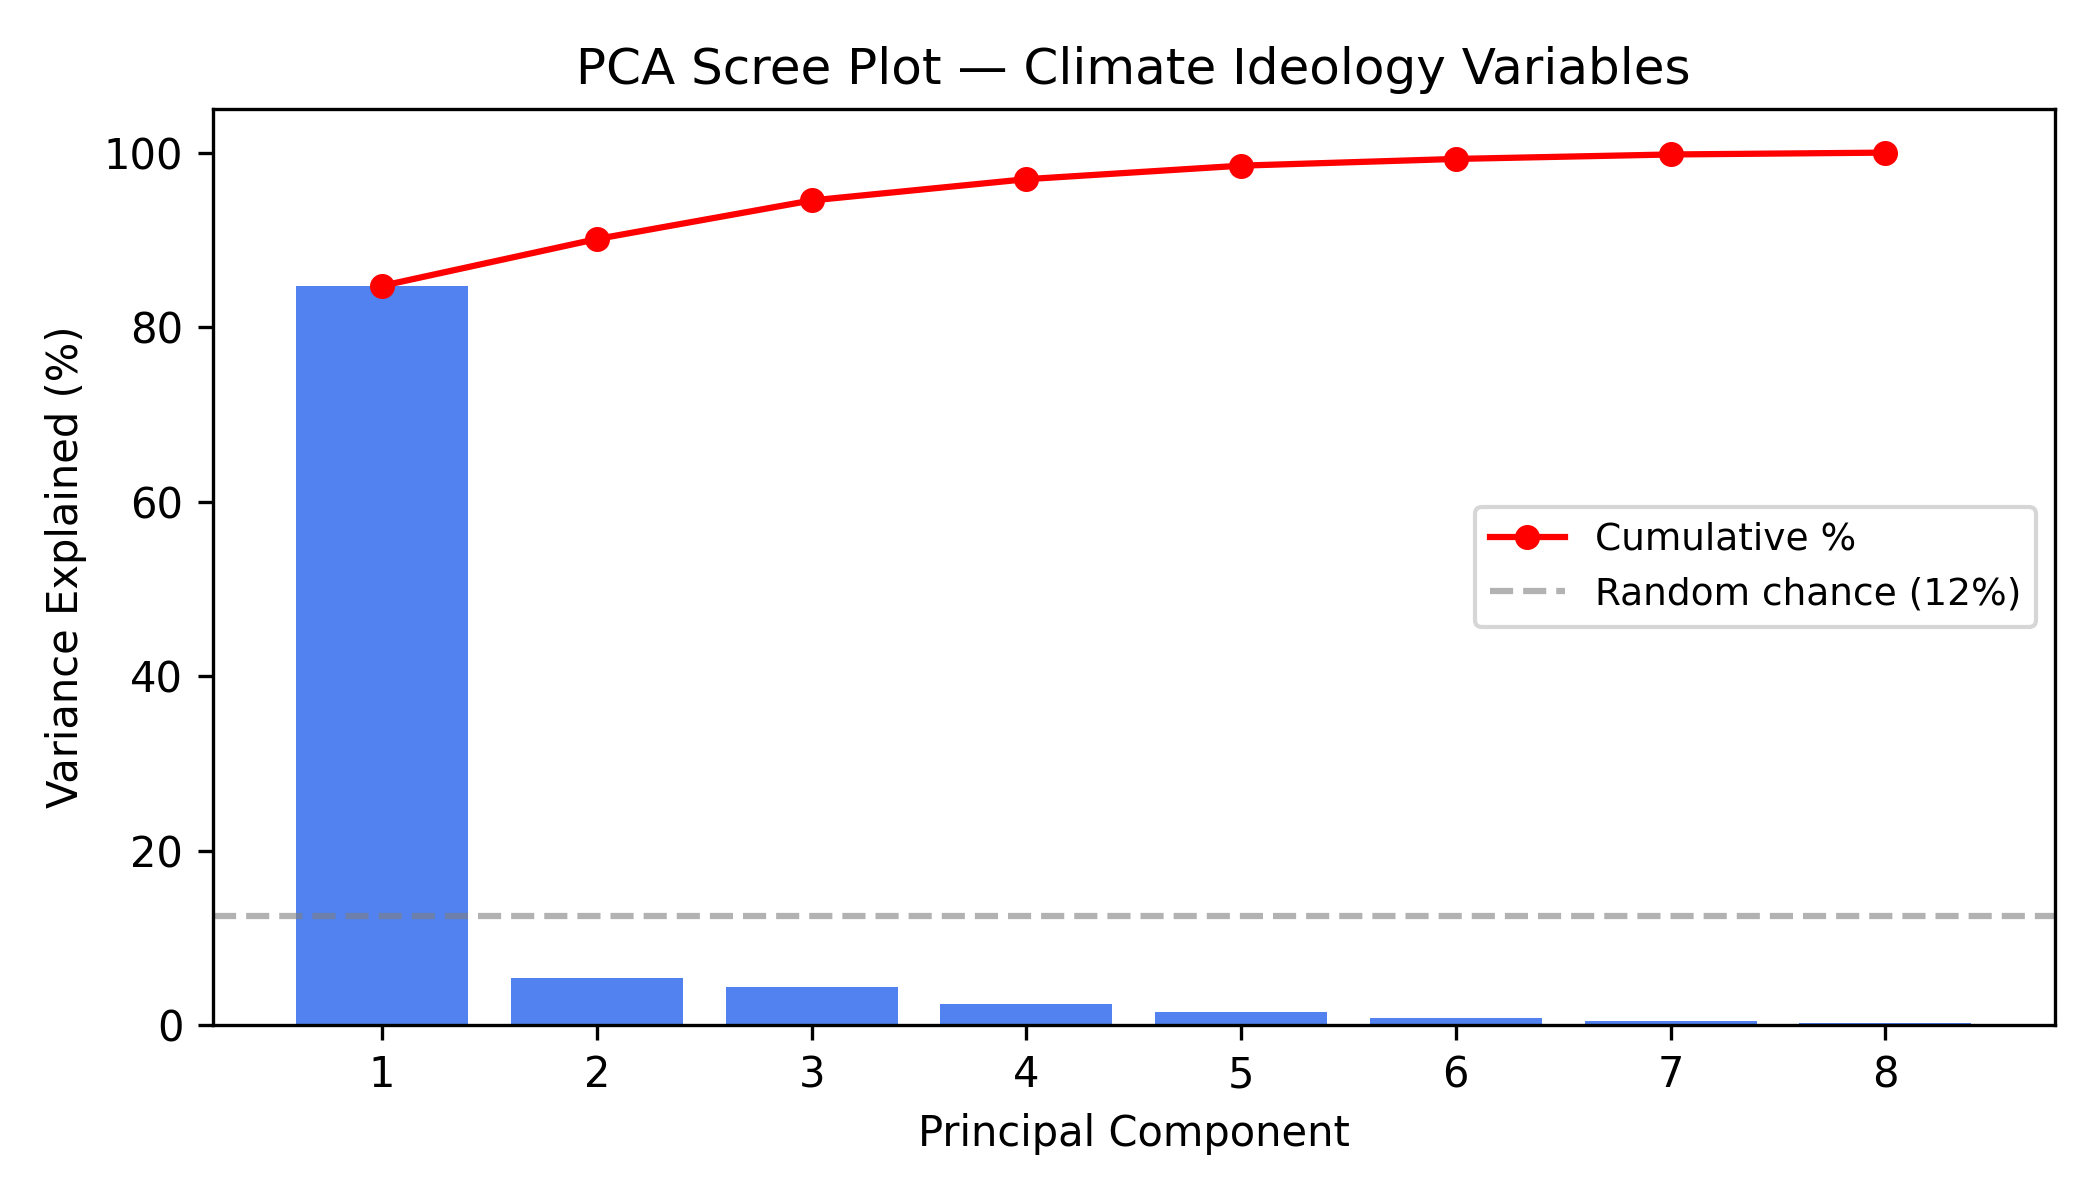
\includegraphics[width=\textwidth]{../output/figures/pca_scree.png}
    \end{column}
  \end{columns}
\end{frame}

\begin{frame}{Composite Climate Ideology Index Across California}
  \begin{center}
    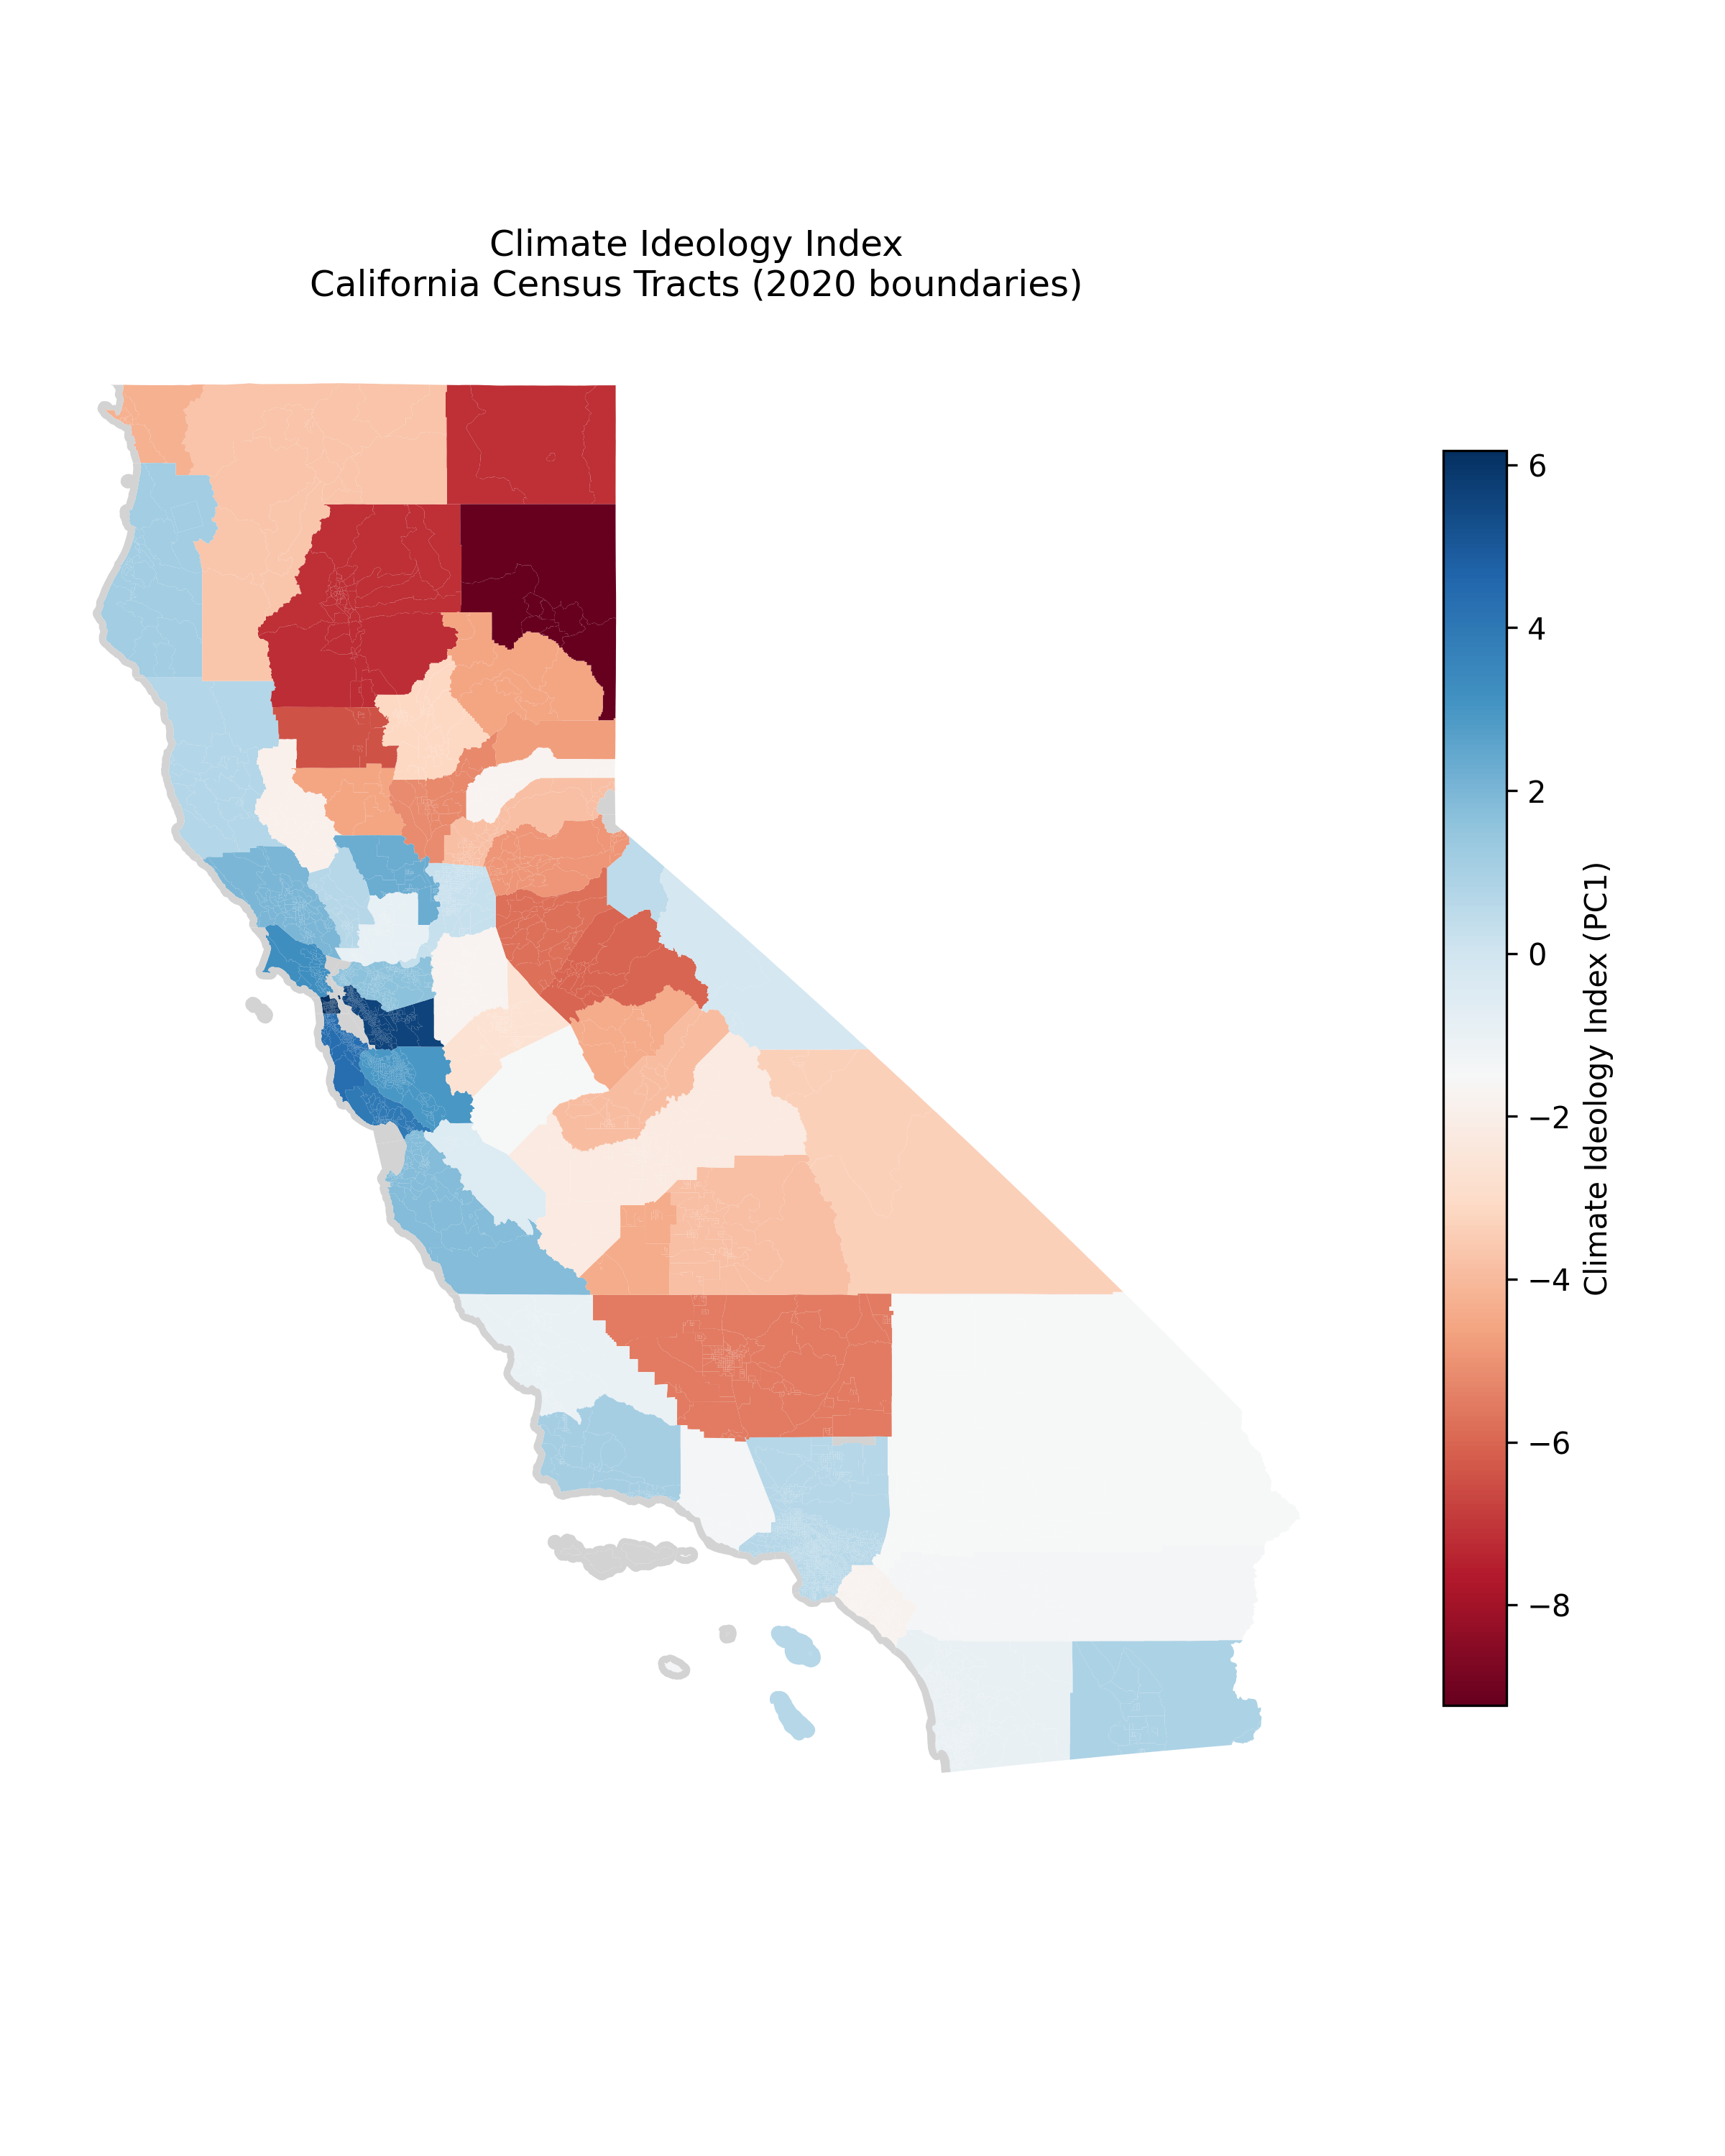
\includegraphics[width=0.82\textwidth]{../output/figures/ideology_map.png}
  \end{center}
  \vspace{-0.3em}
  \src{Climate Ideology Index (PC1, standardized) by Census tract/county. Bay Area, LA, and coastal urban corridors score highest; Central Valley and inland areas score lowest.}
\end{frame}

\begin{frame}{Identification Strategy}
  \begin{columns}[T]
    \begin{column}{0.48\textwidth}
      \textbf{Cross-section (Script 07):}
      \begin{itemize}
        \item OLS: commute behavior $\sim$ ideology + controls
        \item Log-OLS: $\log(\text{BEV}+1)$ $\sim$ ideology + controls
        \item 2023 ACS vintage; HC3 robust SEs
        \item N = 9,003 CA Census tracts
      \end{itemize}

      \vspace{0.8em}
      \textbf{Panel (Script 08):}
      \begin{itemize}
        \item Tract $\times$ year panel, 2018--2024
        \item Year FE absorbs secular EV trends
        \item \textit{Note:} full two-way FE infeasible — ideology is time-invariant; tract FE would absorb it entirely
        \item Ideology identified from cross-sectional variation
        \item Tract-clustered SEs
      \end{itemize}
    \end{column}
    \begin{column}{0.48\textwidth}
      \textbf{Event study (Script 09):}
      \begin{itemize}
        \item Within-tract demeaning (FWL) absorbs tract FE
        \item Ideology $\times$ year interactions estimated relative to 2018 baseline
        \item Events of interest:
          \begin{itemize}
            \item Oct 2022: Musk acquires Twitter
            \item Nov 2024: DOGE / Trump role
          \end{itemize}
        \item Balanced panel: all 7 years, 9,003 tracts
        \item Non-Tesla BEVs as within-time placebo
      \end{itemize}
      \vspace{0.5em}
      \begin{alertblock}{Ecological inference}
        Unit of analysis is the Census tract, not the individual. We observe community-level correlations, not household decisions.
      \end{alertblock}
    \end{column}
  \end{columns}
\end{frame}

% ── Section 3: Results ─────────────────────────────────────────────────────────
\section{Results}

\begin{frame}{Kahn (2007) vs.\ 2025: Side-by-Side}
  \begin{center}
  \begin{tabular}{llcc}
    \toprule
    & & \textbf{Kahn (2007)} & \textbf{Vaughn \& Morehouse (2025)} \\
    \midrule
    \textbf{Ideology proxy} & & Green Party share & Climate Ideology Index (PCA) \\
    \textbf{Geography} & & LA County & Statewide CA \\
    \textbf{Period} & & 2000--2005 & 2018--2024 \\
    \textbf{Method} & & OLS + Neg.\ Binomial & OLS + Year-FE panel \\
    \midrule
    \multicolumn{4}{l}{\textit{Commute behavior:}} \\
    \quad Transit share & & $\uparrow$ sig. & $\uparrow$ +1.09 pp*** \\
    \quad Drive-alone share & & $\downarrow$ sig. & $\downarrow$ $-$1.84 pp*** \\
    \quad Gasoline consumption & & $\downarrow$ sig. & \textit{(not estimated)} \\
    \midrule
    \multicolumn{4}{l}{\textit{Vehicle ownership:}} \\
    \quad Green vehicle (Prius/Tesla) & & $\uparrow$ sig. & $\uparrow$ +5.0\%*** \\
    \quad Non-Tesla EV & & \textit{(pre-EV era)} & $\uparrow$ +6.1\%*** \\
    \quad High-emissions vehicle & & $\downarrow$ sig. & $\downarrow$ $-$2.3\%*** \\
    \midrule
    \multicolumn{4}{l}{\textit{New finding:}} \\
    \quad Elon Effect (post-2022) & & \textit{(n/a)} & \textbf{Not detected through 2024} \\
    \bottomrule
  \end{tabular}
  \end{center}
  \src{Kahn direction/significance from Kahn (2007) Tables 4--6. Our coefficients: per SD of Climate Ideology Index. *** p$<$0.01.}
\end{frame}

\begin{frame}{Replication: Commute Behavior (Cross-Section, 2023)}
  \begin{columns}[T]
    \begin{column}{0.48\textwidth}
      \textbf{Transit commute share}\\
      \src{OLS, HC3 robust SEs, N=9,003 tracts}

      \vspace{0.4em}
      \begin{tabular}{lcc}
        \toprule
        \textbf{Variable} & \textbf{Coef} & \textbf{SE} \\
        \midrule
        \sig{Ideology index} & \sig{+0.0109***} & \sig{(0.0003)} \\
        log(HH income) & $-$0.0448*** & (0.0024) \\
        \% BA+ & +0.0945*** & (0.0072) \\
        Pop.\ density & $-$0.000*** & (0.000) \\
        \% White & $-$0.0310*** & (0.0025) \\
        \% WFH & +0.0232*** & (0.0079) \\
        \midrule
        $R^2$ & \multicolumn{2}{c}{0.341} \\
        \bottomrule
      \end{tabular}
    \end{column}
    \begin{column}{0.48\textwidth}
      \textbf{Drive-alone commute share}\\
      \src{OLS, HC3 robust SEs, N=9,003 tracts}

      \vspace{0.4em}
      \begin{tabular}{lcc}
        \toprule
        \textbf{Variable} & \textbf{Coef} & \textbf{SE} \\
        \midrule
        \sig{Ideology index} & \sig{$-$0.0184***} & \sig{(0.0006)} \\
        log(HH income) & +0.1017*** & (0.0040) \\
        \% BA+ & $-$0.1134*** & (0.0154) \\
        Pop.\ density & +0.000** & (0.000) \\
        \% White & +0.0456*** & (0.0054) \\
        \% WFH & $-$0.8806*** & (0.0154) \\
        \midrule
        $R^2$ & \multicolumn{2}{c}{0.594} \\
        \bottomrule
      \end{tabular}
    \end{column}
  \end{columns}
  \vspace{0.5em}
  \textbf{Interpretation:} 1 SD $\uparrow$ ideology $\Rightarrow$ +1.09 pp transit, $-$1.84 pp drive-alone.
  Given average shares of $\approx$5\% transit and $\approx$76\% drive-alone, these are economically meaningful.
\end{frame}

\begin{frame}{EV Panel Results (2018--2024)}
  \begin{columns}[T]
    \begin{column}{0.48\textwidth}
      \begin{tabular}{lccc}
        \toprule
        \textbf{Outcome} & \textbf{Coef} & \textbf{SE} & \textbf{$R^2$} \\
        \midrule
        log(Tesla+1) & +0.0495*** & (0.0051) & 0.619 \\
        log(non-Tesla BEV+1) & +0.0605*** & (0.0046) & 0.492 \\
        log(light truck+1) & $-$0.0226*** & (0.0058) & 0.130 \\
        Tesla share of BEVs & +0.0022*** & (0.0008) & 0.521 \\
        \bottomrule
      \end{tabular}
      \src{Year FE, tract-clustered SEs. N=63,021 (9,003 tracts $\times$ 7 years).\\
      Controls: log income, \% BA+, pop density, \% white, \% WFH.}

      \vspace{0.5em}
      \textbf{Key results:}
      \begin{itemize}
        \item 1 SD ideology $\Rightarrow$ +5.0\% Teslas, +6.1\% non-Tesla EVs
        \item High-ideology tracts have \textit{fewer} light trucks ($-$2.3\%)
        \item High-ideology tracts also have a \textit{higher Tesla share} within the EV fleet
      \end{itemize}
    \end{column}
    \begin{column}{0.48\textwidth}
      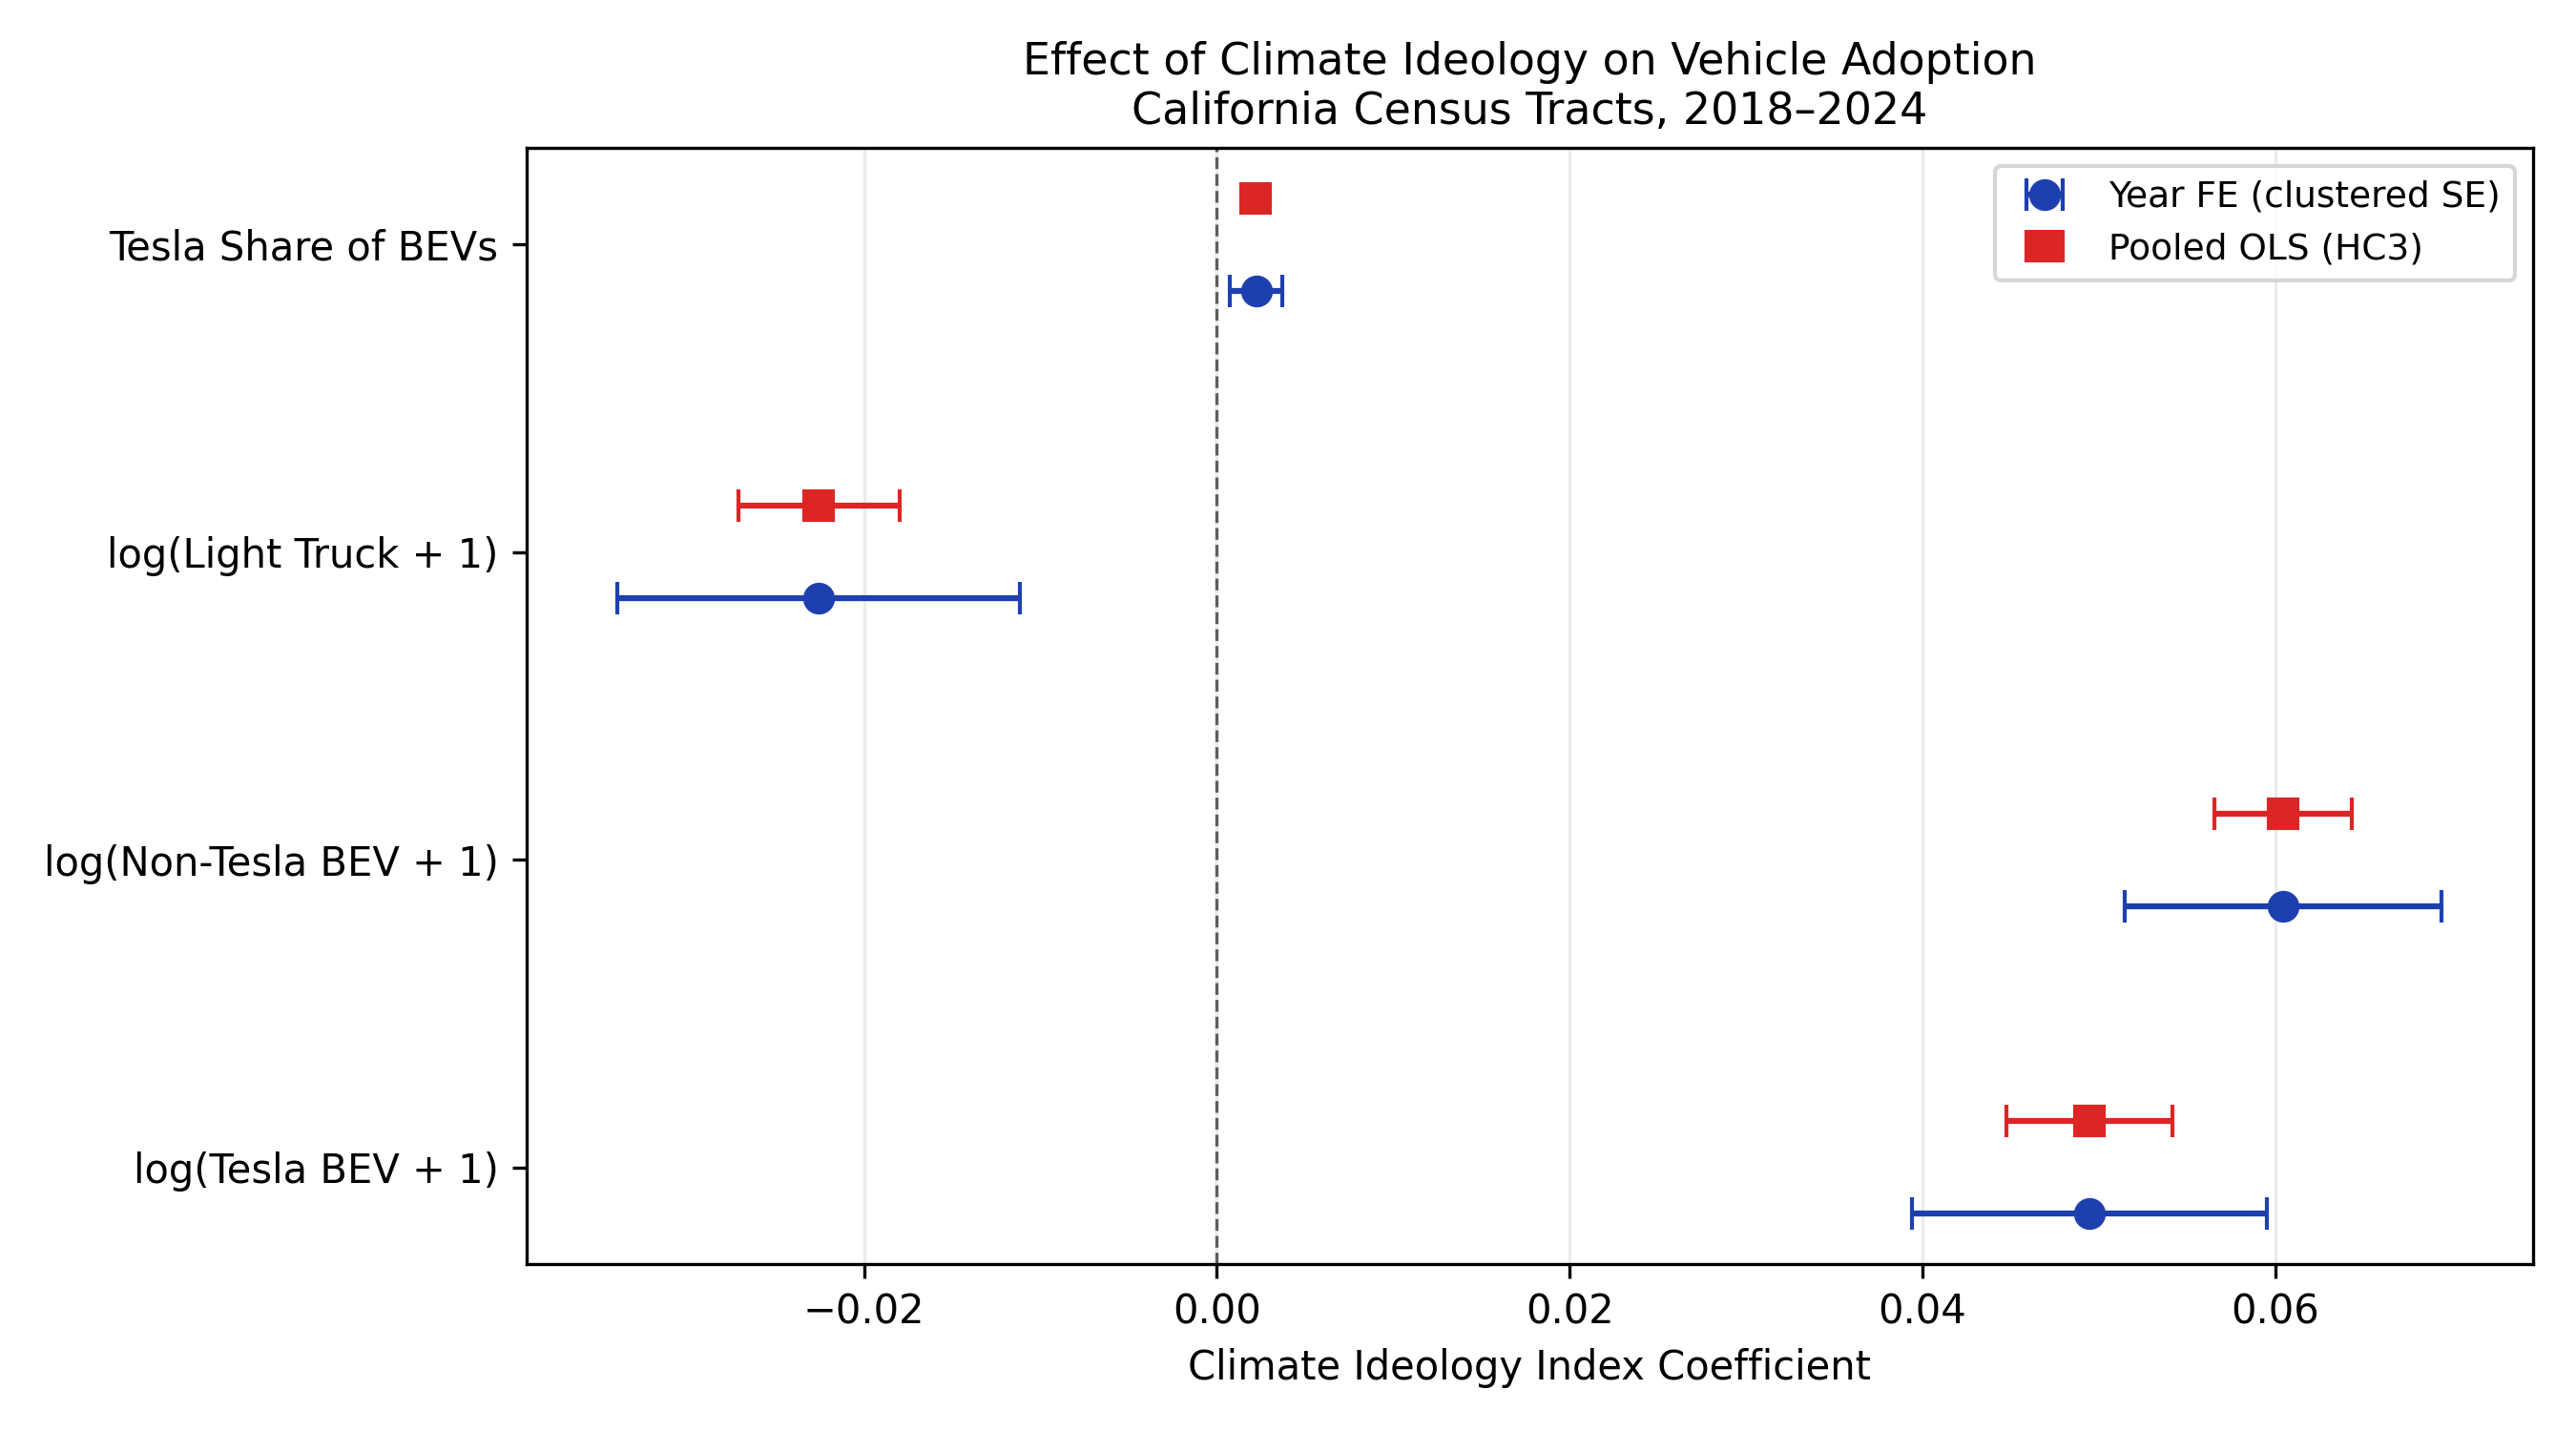
\includegraphics[width=\textwidth]{../output/figures/ev_panel_coefs.png}
      \src{Ideology coefficient by vehicle type, year FE model. 95\% CI from tract-clustered SEs.}
    \end{column}
  \end{columns}
\end{frame}

\begin{frame}{The Elon Effect}
  \begin{center}
    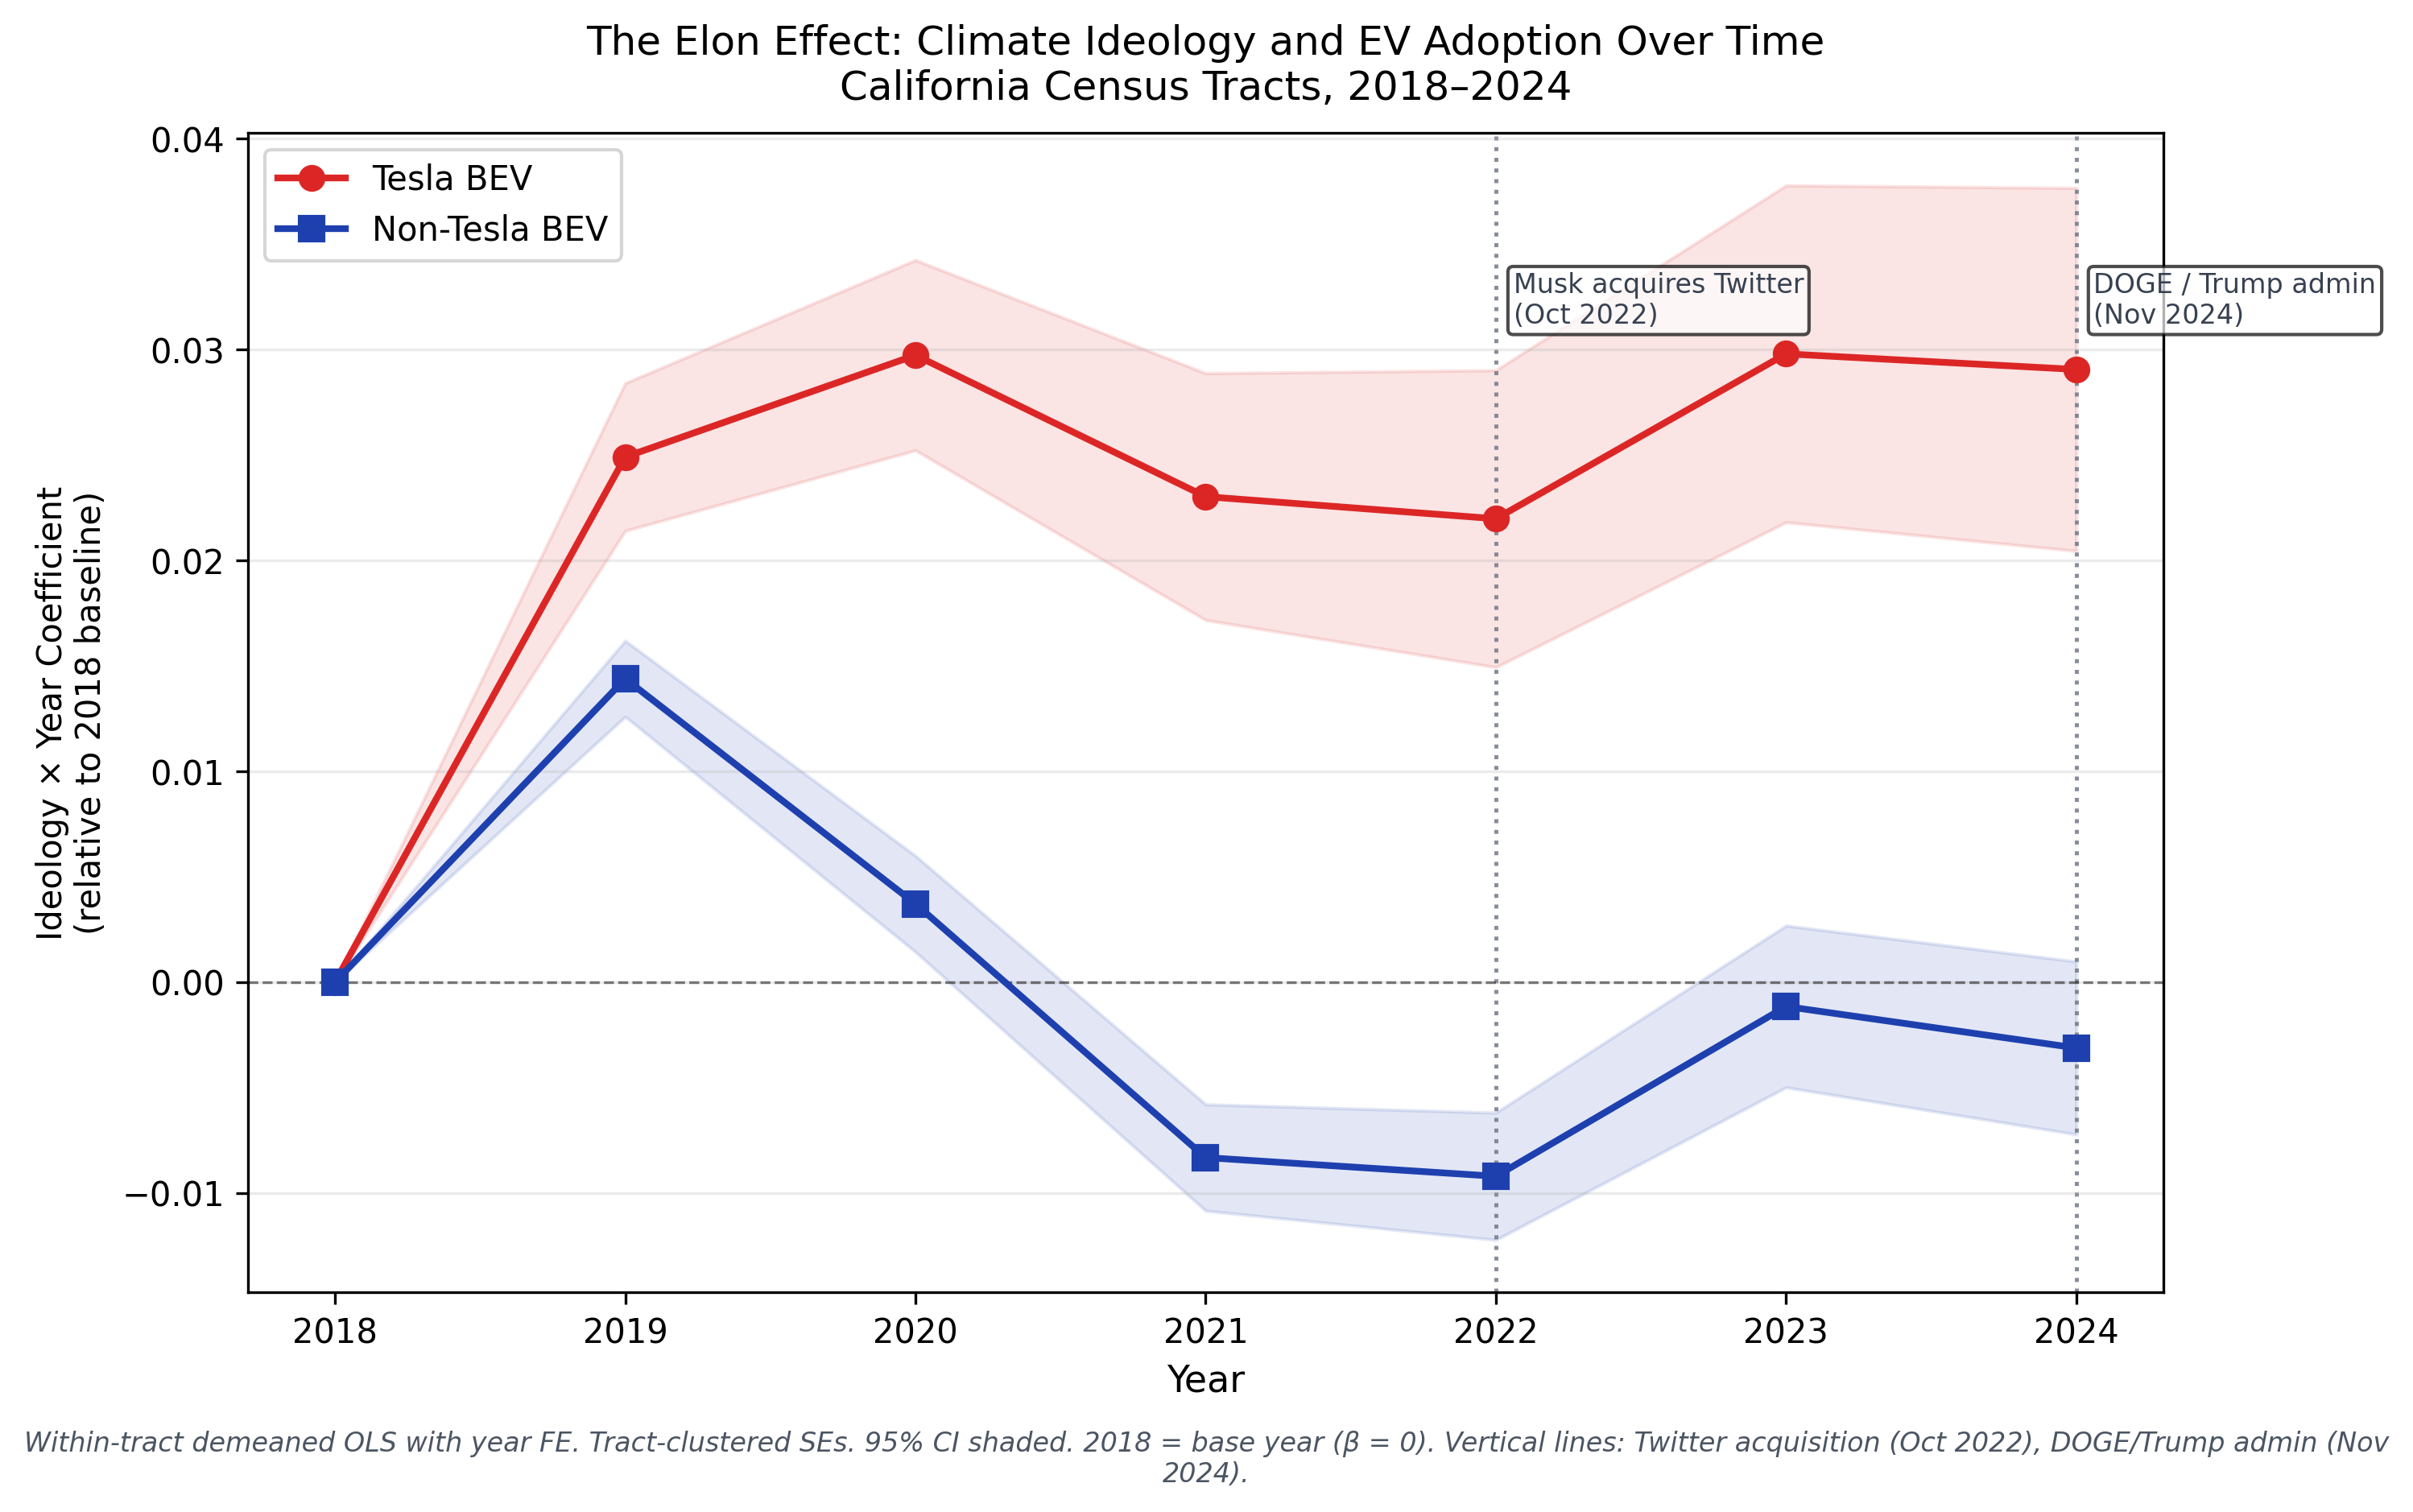
\includegraphics[width=0.82\textwidth]{../output/figures/event_study_tesla_vs_nontesla.png}
  \end{center}
  \vspace{-0.4em}
  \src{Ideology $\times$ year interaction coefficients relative to 2018. Within-tract demeaned OLS; tract-clustered SEs; 95\% CI shaded.
  Vertical dotted lines: Musk Twitter acquisition (Oct 2022) and DOGE/Trump role (Nov 2024).}
\end{frame}

\begin{frame}{The Elon Effect: Interpretation}
  \begin{columns}[T]
    \begin{column}{0.55\textwidth}
      \textbf{What the event study shows:}

      \vspace{0.5em}
      \textcolor{elonred}{\textbf{Tesla (red):}}
      \begin{itemize}
        \item Ideology--Tesla link \textit{strengthened} 2018$\to$2020 (+0.025 to +0.030)
        \item Held broadly \textit{flat} through 2024 (+0.022 to +0.030)
        \item \textbf{No clear post-2022 decline}
      \end{itemize}

      \vspace{0.5em}
      \textcolor{evblue}{\textbf{Non-Tesla BEV (blue):}}
      \begin{itemize}
        \item Rose in 2019 (+0.014), then \textit{fell below baseline} 2021--2022 ($-$0.008 to $-$0.009)
        \item Recovered by 2023--2024
        \item Interpretation: \textbf{market democratization} — Bolt/Leaf/Ioniq spread into lower-ideology communities as prices fell
      \end{itemize}
    \end{column}
    \begin{column}{0.42\textwidth}
      \begin{alertblock}{What this does NOT show}
        \begin{itemize}
          \item The most dramatic Musk political events (DOGE, Trump administration) only appear at the \textbf{tail of the 2024 panel}
          \item The data window is too short to detect a shift that may be emerging now
          \item 2025 CEC data (not yet available) is needed for a definitive test
        \end{itemize}
      \end{alertblock}
      \vspace{0.5em}
      \begin{block}{Placebo check}
        Light truck ideology coefficients move separately and monotonically — not confounded with the EV story.
      \end{block}
    \end{column}
  \end{columns}
\end{frame}

% ── Section 4: Conclusions ─────────────────────────────────────────────────────
\section{Conclusions}

\begin{frame}{Conclusions}
  \begin{enumerate}
    \item \textbf{Kahn's finding survives into the EV era.} Climate ideology robustly predicts lower-carbon commuting behavior and higher EV ownership in 2023 California. The green signal is alive.

    \vspace{0.5em}
    \item \textbf{Non-Tesla EVs are democratizing.} The ideology--non-Tesla-EV link weakened 2020--2022 as affordable models spread beyond high-ideology communities. The technology is outrunning the brand signal.

    \vspace{0.5em}
    \item \textbf{The Elon Effect is not yet detectable.} The Tesla--ideology link remained stable through 2024. But the data window may be too short: the most consequential Musk political events appear only at the tail of our panel.

    \vspace{0.5em}
    \item \textbf{Spatial autocorrelation is strong but does not reverse results.} Moran's I = 0.58 (transit); SAR $\hat{\rho}$ = 0.78. Ideology coefficients survive spatial correction.

    \vspace{0.5em}
    \item \textbf{All main results robust} to three alternative ideology specifications (YCOM-only, no-YCOM, Prop 30 alone).
  \end{enumerate}
\end{frame}

\begin{frame}{Next Steps}
  \begin{columns}[T]
    \begin{column}{0.48\textwidth}
      \textbf{High priority:}
      \begin{enumerate}
        \item \textbf{2025 CEC data} — when available, re-run event study with DOGE/Trump window fully in sample; this is the definitive Elon Effect test
        \item \textbf{AFDC EV charger density} — acquire from DOE AFDC API and add as a control; currently omitted despite being a meaningful EV adoption confounder
        \item \textbf{Time-varying ACS controls} — use 2019 ACS (2015--2019 5-year, 2010 tract definitions) for 2018--2020 panel years via NHGIS crosswalk; removes time-invariant control assumption
      \end{enumerate}
    \end{column}
    \begin{column}{0.48\textwidth}
      \textbf{Extensions:}
      \begin{enumerate}
        \setcounter{enumi}{3}
        \item \textbf{National replication} — extend beyond California; requires state-level ideology proxies (YCOM is national) and DMV-equivalent vehicle data
        \item \textbf{Individual-level data} — address the ecological inference limitation with household-level vehicle or survey data; California NHTS subsample or CA DMV microdata
        \item \textbf{Brand-level heterogeneity} — decompose non-Tesla EVs by brand (Chevy Bolt vs.\ Rivian vs.\ Hyundai); different price points may have distinct ideology profiles
        \item \textbf{Publish} — fill GitHub link, post to Substack, submit to NBER EEE working paper series
      \end{enumerate}
    \end{column}
  \end{columns}
\end{frame}

% ══════════════════════════════════════════════════════════════════════════════
\appendix
% ══════════════════════════════════════════════════════════════════════════════

\begin{frame}{Appendix: Contents}
  \tableofcontents[sectionstyle=show,hideallsubsections]
  \vspace{0.5em}
  \begin{itemize}
    \item[A1--A2] Robustness checks: alternative ideology specifications
    \item[A3] Spatial diagnostics (Moran's I and SAR)
    \item[A4--A11] Ideology component maps across California
    \item[A12] Placebo check: light truck event study
  \end{itemize}
\end{frame}

% ── Appendix A: Robustness ─────────────────────────────────────────────────────

\begin{frame}{A1: Robustness — Transit Commute Share}
  \begin{center}
  \begin{tabular}{llcccc}
    \toprule
    \textbf{Spec} & \textbf{Ideology measure} & \textbf{Coef} & \textbf{SE} & \textbf{$R^2$} & \textbf{N} \\
    \midrule
    Main    & PCA composite (all 8)  & +0.0109*** & (0.0003) & 0.341 & 9,003 \\
    R1      & YCOM PCA only          & +0.0011    & (0.0023) & 0.503 & 58 \\
    R2      & Voter reg + ballot PCA & +0.0173*** & (0.0005) & 0.351 & 9,003 \\
    R3      & Prop 30 share only     & +0.3920*** & (0.0133) & 0.354 & 9,003 \\
    \bottomrule
  \end{tabular}
  \end{center}

  \vspace{0.5em}
  \textbf{Notes:}
  \begin{itemize}
    \item R1 insignificance reflects loss of power at county level (N=58), not reversal of direction
    \item R2 and R3 are \textit{stronger} than Main — electoral behavior is a particularly tight predictor of commute patterns at tract level
    \item R1 county controls use unweighted tract means; interpret R1 estimates for heterogeneous counties with caution
  \end{itemize}
\end{frame}

\begin{frame}{A2: Robustness — Drive-Alone Commute Share}
  \begin{center}
  \begin{tabular}{llcccc}
    \toprule
    \textbf{Spec} & \textbf{Ideology measure} & \textbf{Coef} & \textbf{SE} & \textbf{$R^2$} & \textbf{N} \\
    \midrule
    Main    & PCA composite (all 8)  & $-$0.0184*** & (0.0006) & 0.594 & 9,003 \\
    R1      & YCOM PCA only          & $-$0.0078**  & (0.0036) & 0.821 & 58 \\
    R2      & Voter reg + ballot PCA & $-$0.0288*** & (0.0009) & 0.596 & 9,003 \\
    R3      & Prop 30 share only     & $-$0.6973*** & (0.0209) & 0.611 & 9,003 \\
    \bottomrule
  \end{tabular}
  \end{center}

  \vspace{0.5em}
  \textbf{Notes:}
  \begin{itemize}
    \item R1 significant at 5\% level despite N=58 — county-level YCOM is precise enough to detect the drive-alone effect
    \item Direction consistent across all four specifications
    \item High $R^2$ in R1 (0.821) reflects both ideology strength and collinearity in county-level controls
  \end{itemize}
\end{frame}

% ── Appendix B: Spatial ───────────────────────────────────────────────────────

\begin{frame}{A3: Spatial Diagnostics}
  \begin{columns}[T]
    \begin{column}{0.48\textwidth}
      \textbf{Moran's I on OLS residuals:}

      \vspace{0.4em}
      \begin{tabular}{lccc}
        \toprule
        \textbf{Model} & \textbf{I} & \textbf{p} & \textbf{Sig?} \\
        \midrule
        Transit share & 0.582 & 0.001 & Yes \\
        Drive-alone   & 0.408 & 0.001 & Yes \\
        \bottomrule
      \end{tabular}
      \src{999 permutations. Queen contiguity weights, 9,003 tracts.}

      \vspace{0.8em}
      \textbf{SAR model ($\hat{\rho}$):}

      \vspace{0.4em}
      \begin{tabular}{lcc}
        \toprule
        \textbf{Model} & \textbf{$\hat{\rho}$} & \textbf{SE} \\
        \midrule
        Transit share & 0.781*** & (0.008) \\
        Drive-alone   & 0.567*** & (0.009) \\
        \bottomrule
      \end{tabular}
      \src{Spatial Lag Model (SAR), ML estimation, queen contiguity.}
    \end{column}
    \begin{column}{0.48\textwidth}
      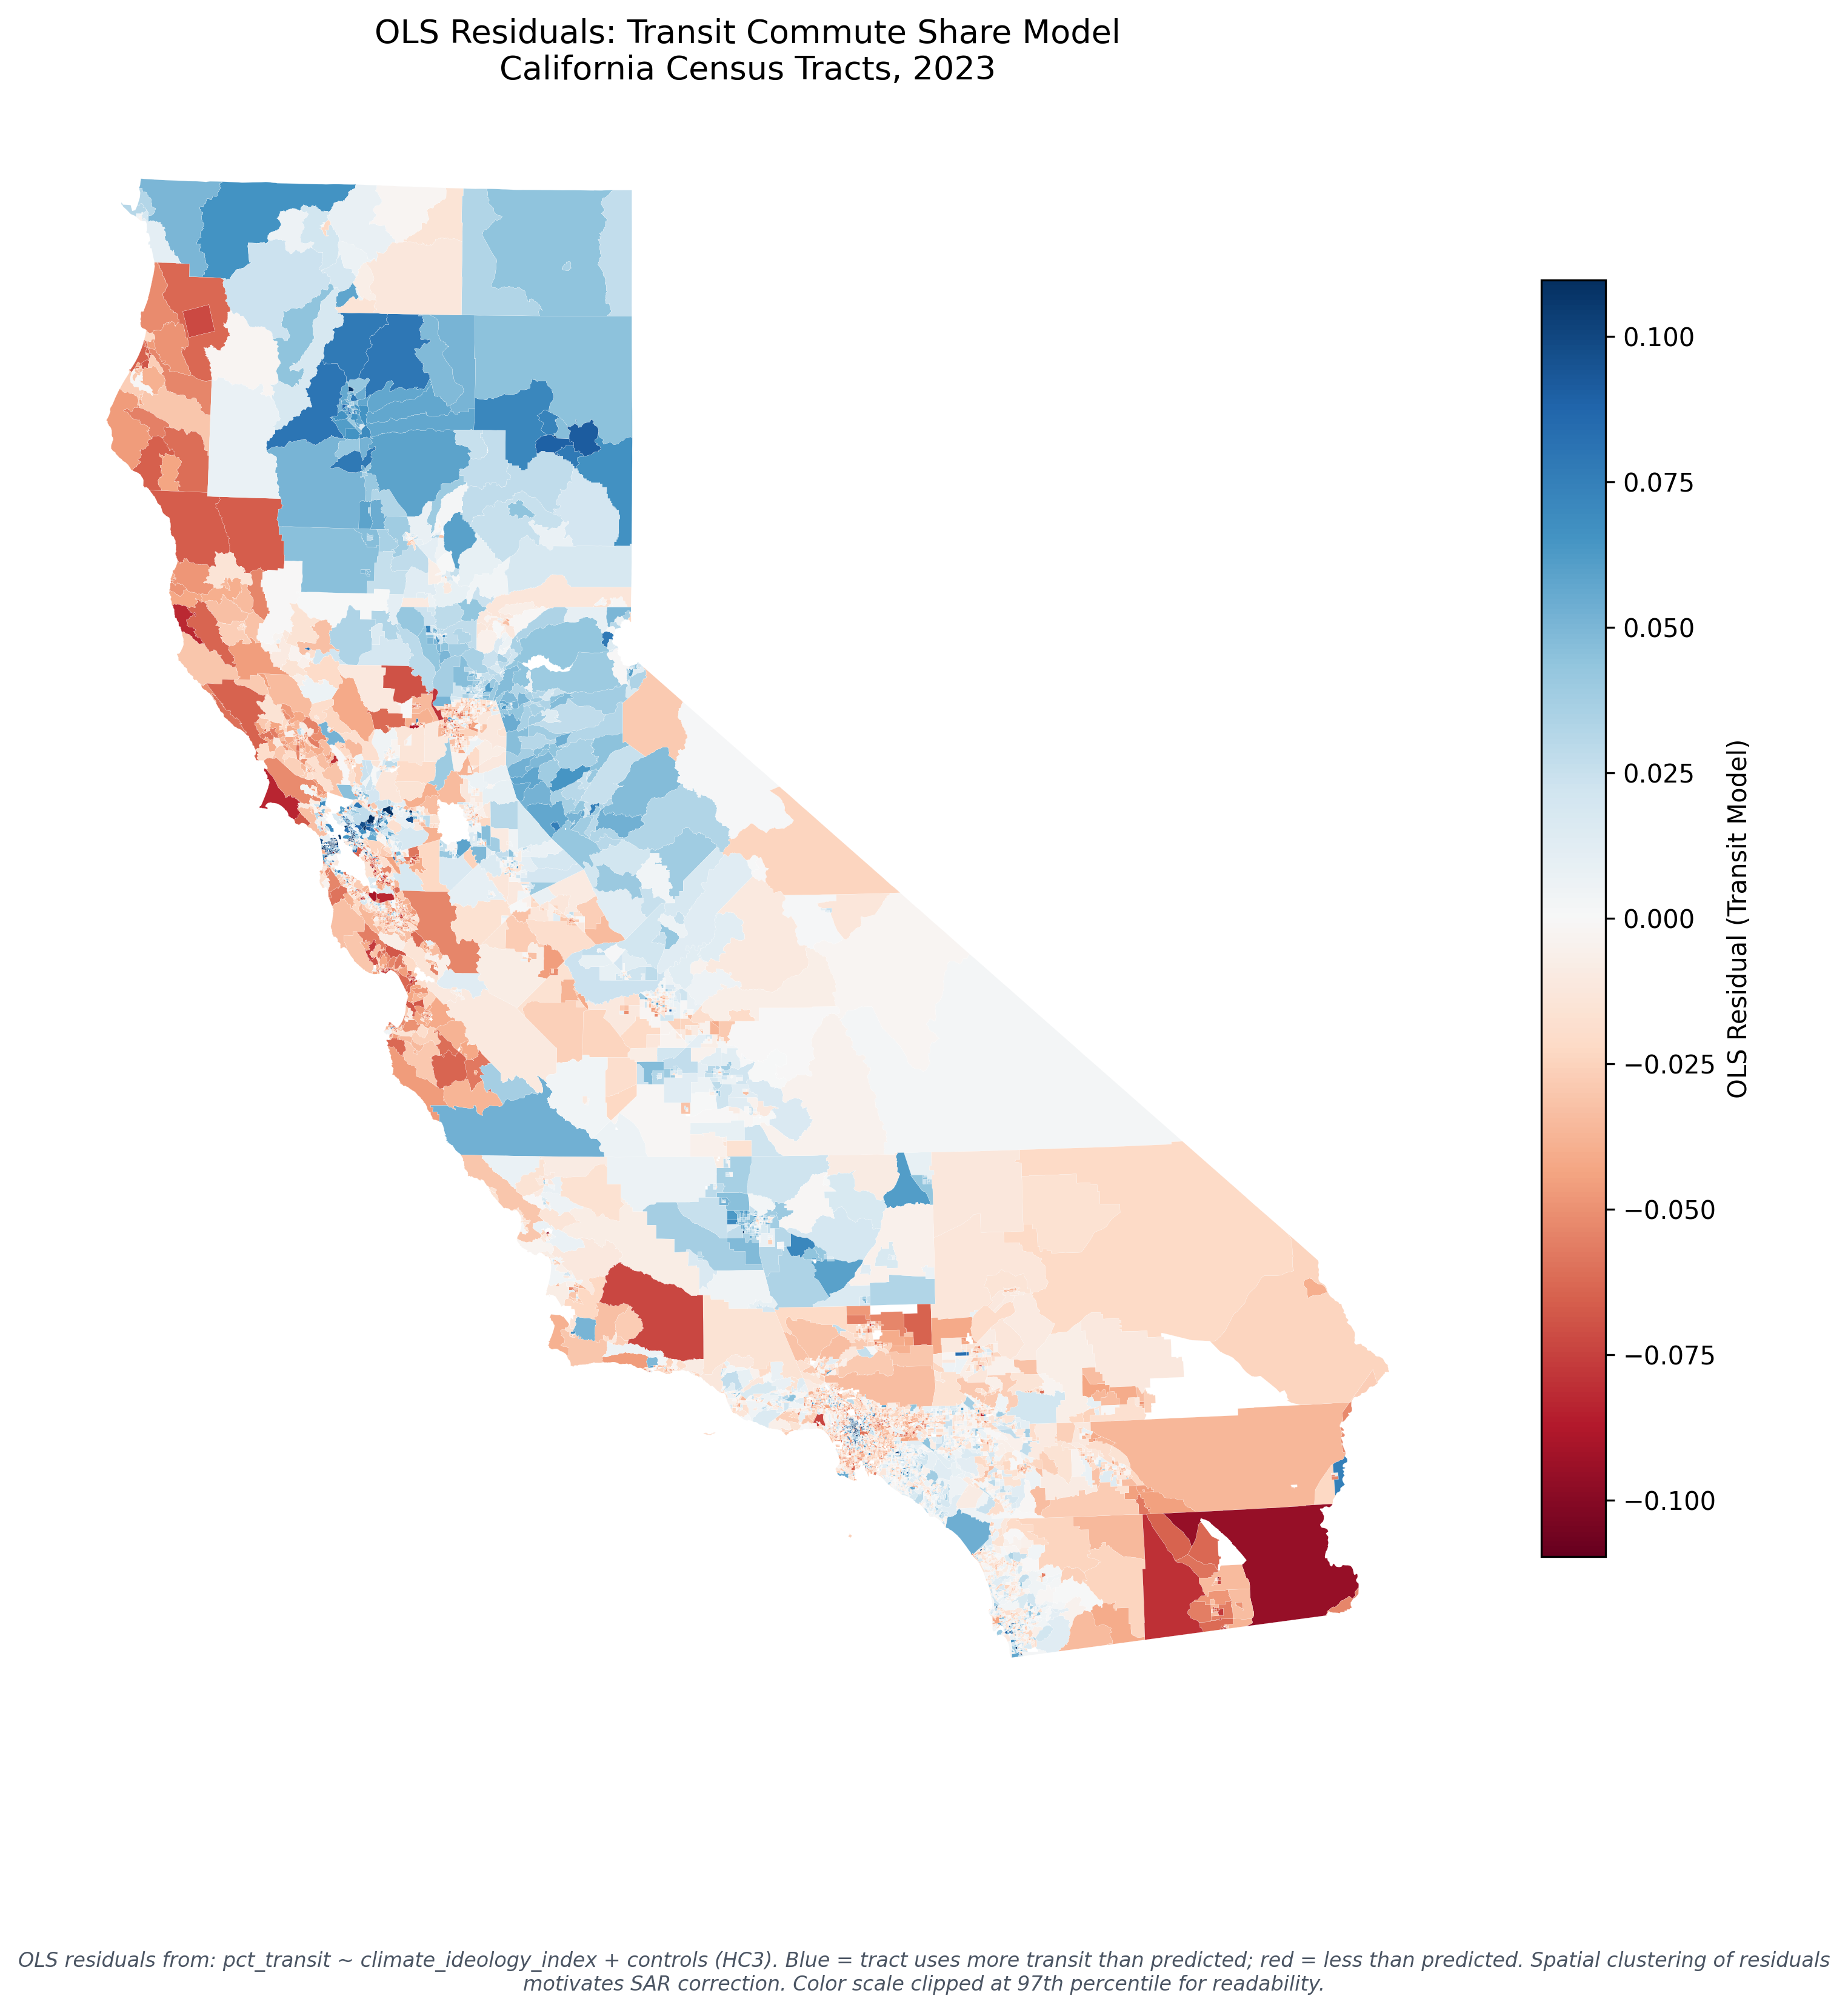
\includegraphics[width=\textwidth]{../output/figures/residual_map.png}
      \src{OLS residuals from transit model. Clustered positive residuals in dense corridors confirm spatial autocorrelation.}

      \vspace{0.5em}
      \textbf{Conclusion:} Strong spatial dependence present — transit access is geographically clustered. Ideology coefficients survive SAR correction.
    \end{column}
  \end{columns}
\end{frame}

% ── Appendix C: Component Maps ────────────────────────────────────────────────

\begin{frame}{A4--A11: Ideology Component Maps — Overview}
  All eight ideology components are measured at the \textbf{county level} (N=58 CA counties) due to SWDB precinct key incompatibility with the Census MPREC system.

  \vspace{0.5em}
  Maps on the following slides show each component as a county choropleth.\\
  Generate all maps by running: \texttt{python scripts/12\_component\_maps.py}

  \vspace{0.8em}
  \begin{tabular}{lll}
    \toprule
    \textbf{Slide} & \textbf{Variable} & \textbf{Source} \\
    \midrule
    A4 & \% Think climate change is happening & YCOM \\
    A5 & \% Worried about climate change & YCOM \\
    A6 & \% Say climate change is human-caused & YCOM \\
    A7 & \% Support regulation & YCOM \\
    A8 & \% Support Renewable Portfolio Standard & YCOM \\
    A9 & Democrat $-$ Republican registration share & CA SoS \\
    A10 & Prop 30 YES share (2022, EV/wildfire funding) & CA SoS / SWDB \\
    A11 & Prop 68 YES share (2018, environmental bonds) & CA SoS / SWDB \\
    \bottomrule
  \end{tabular}
\end{frame}

\begin{frame}{A4: \% Think Climate Change Is Happening (YCOM, County Level)}
  \begin{center}
    \IfFileExists{../output/figures/map_ycom_happening.png}{%
      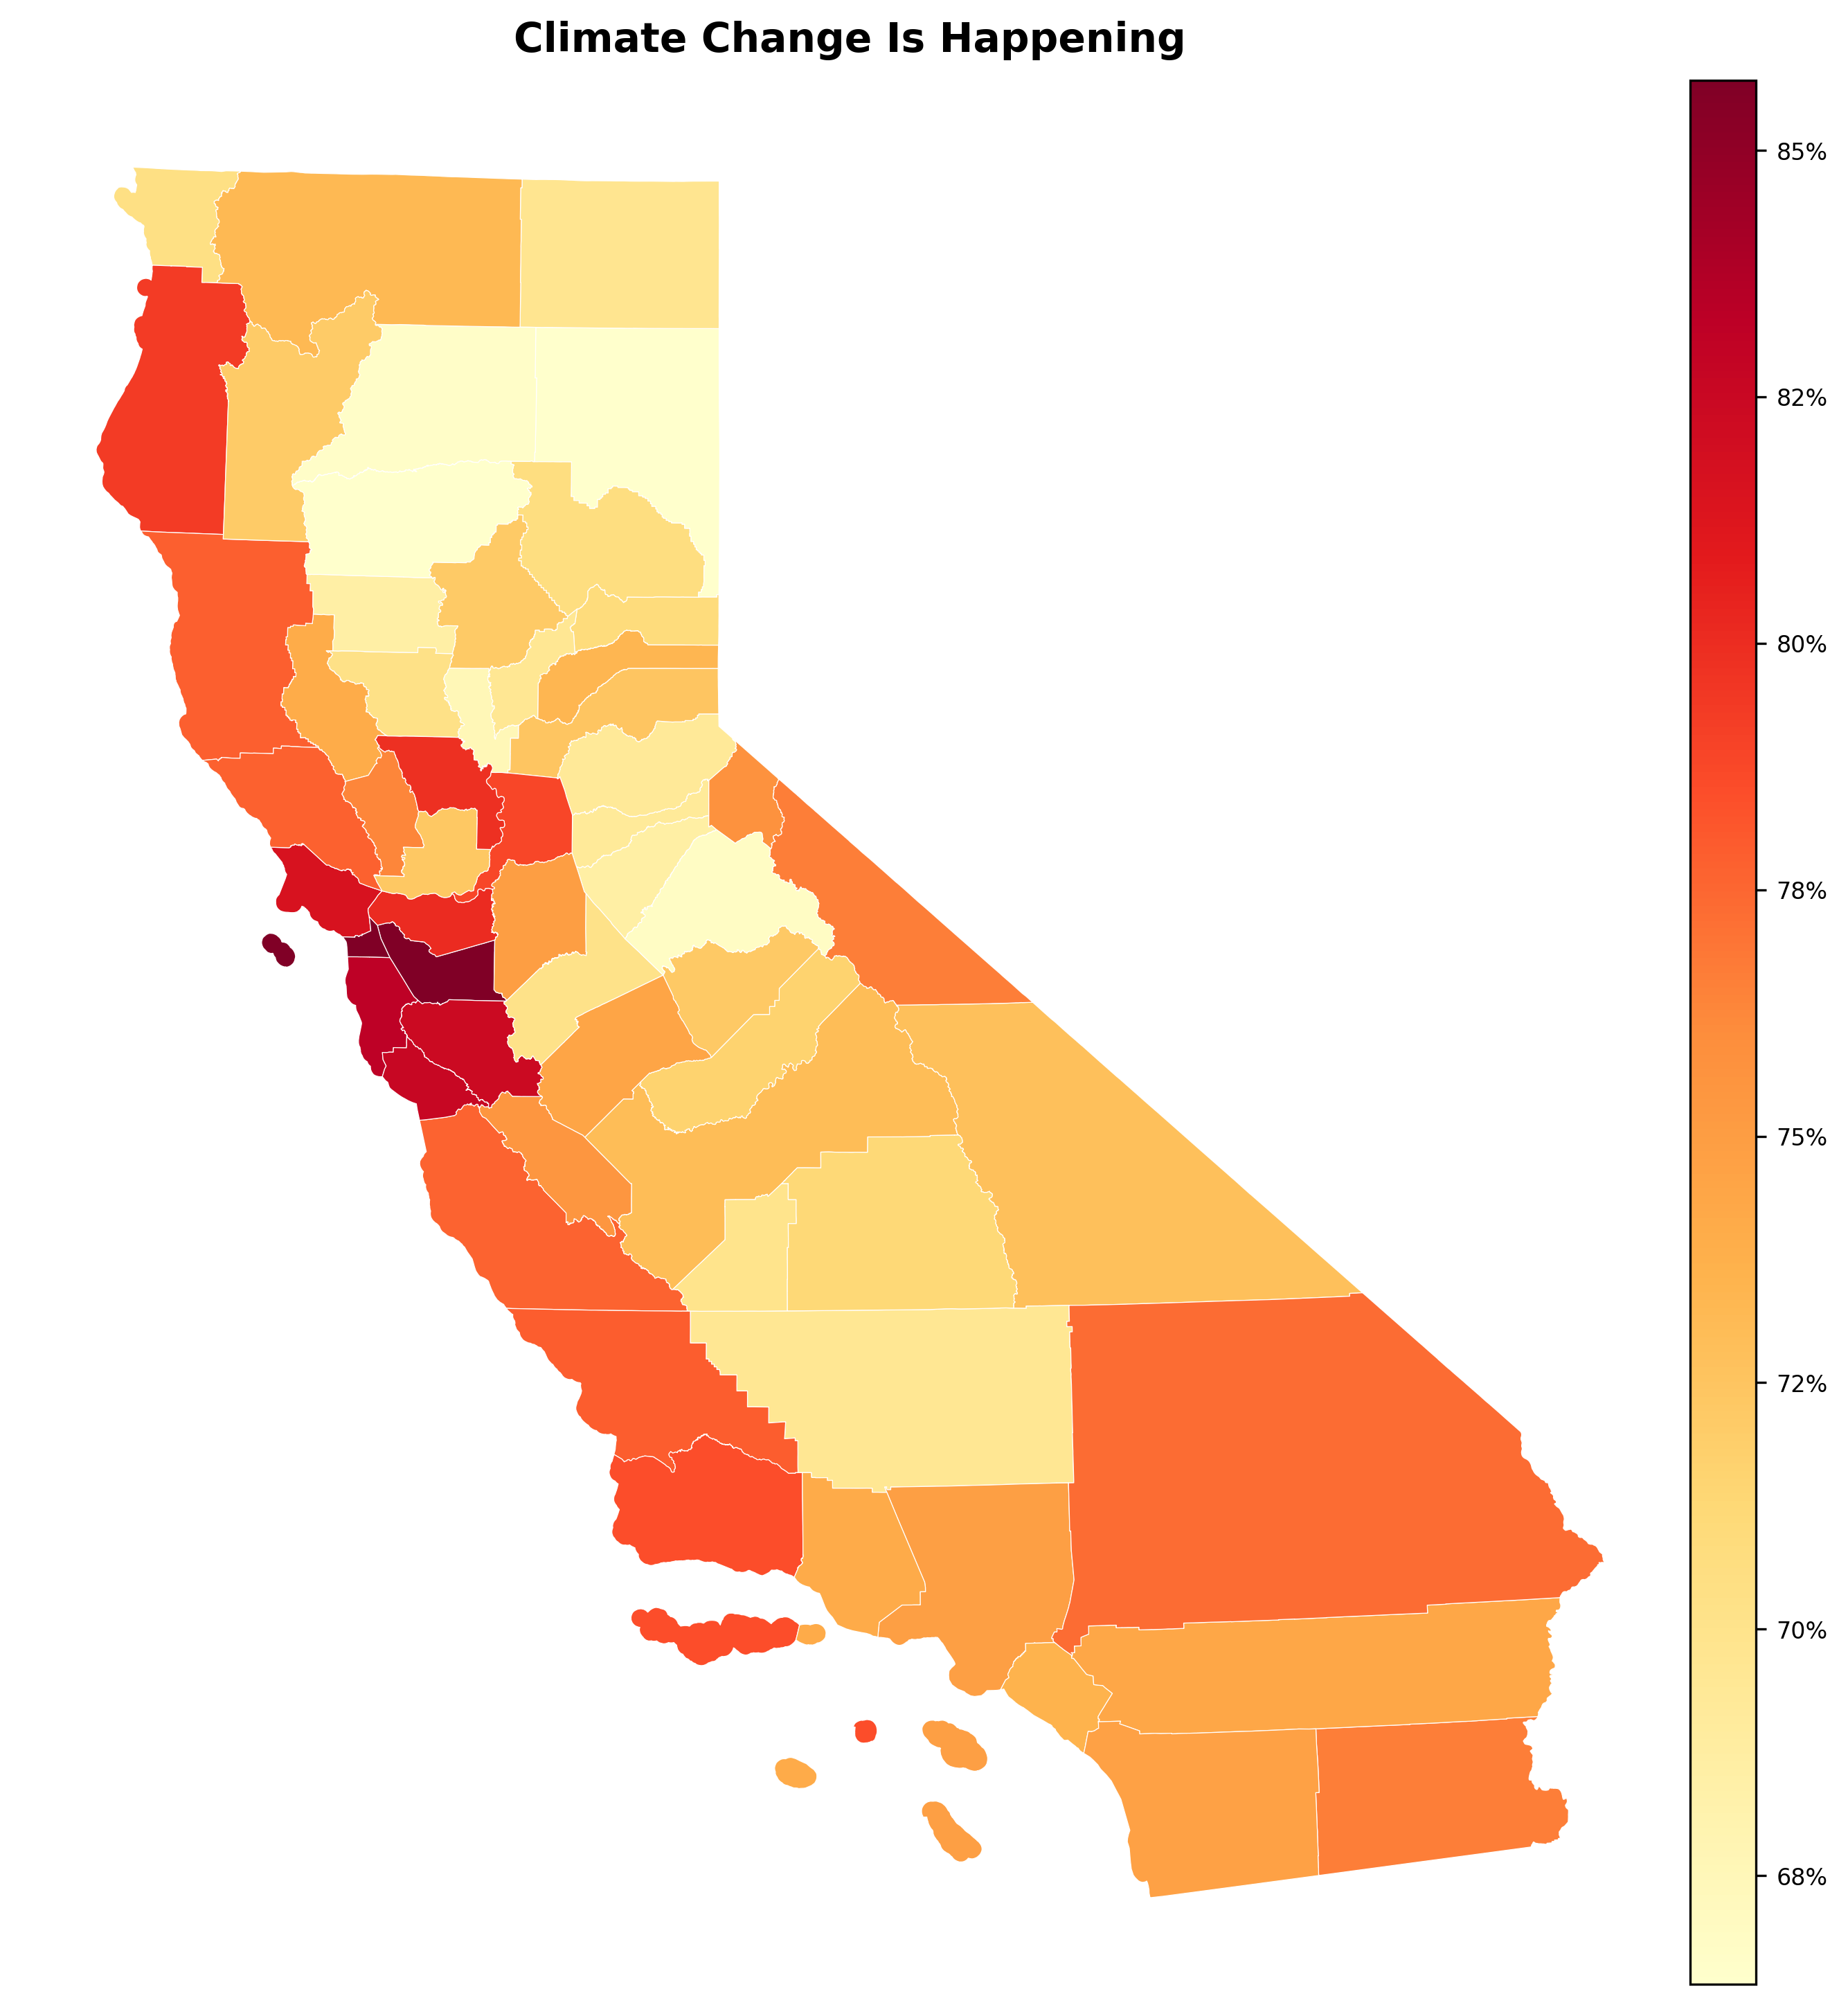
\includegraphics[width=0.80\textwidth]{../output/figures/map_ycom_happening.png}
    }{%
      \missingfig{map\_ycom\_happening.png}
    }
  \end{center}
  \src{Yale Climate Opinion Maps (YCOM), 2023. County-level MrP estimates. \% of county residents who agree that climate change is happening.}
\end{frame}

\begin{frame}{A5: \% Worried About Climate Change (YCOM, County Level)}
  \begin{center}
    \IfFileExists{../output/figures/map_ycom_worried.png}{%
      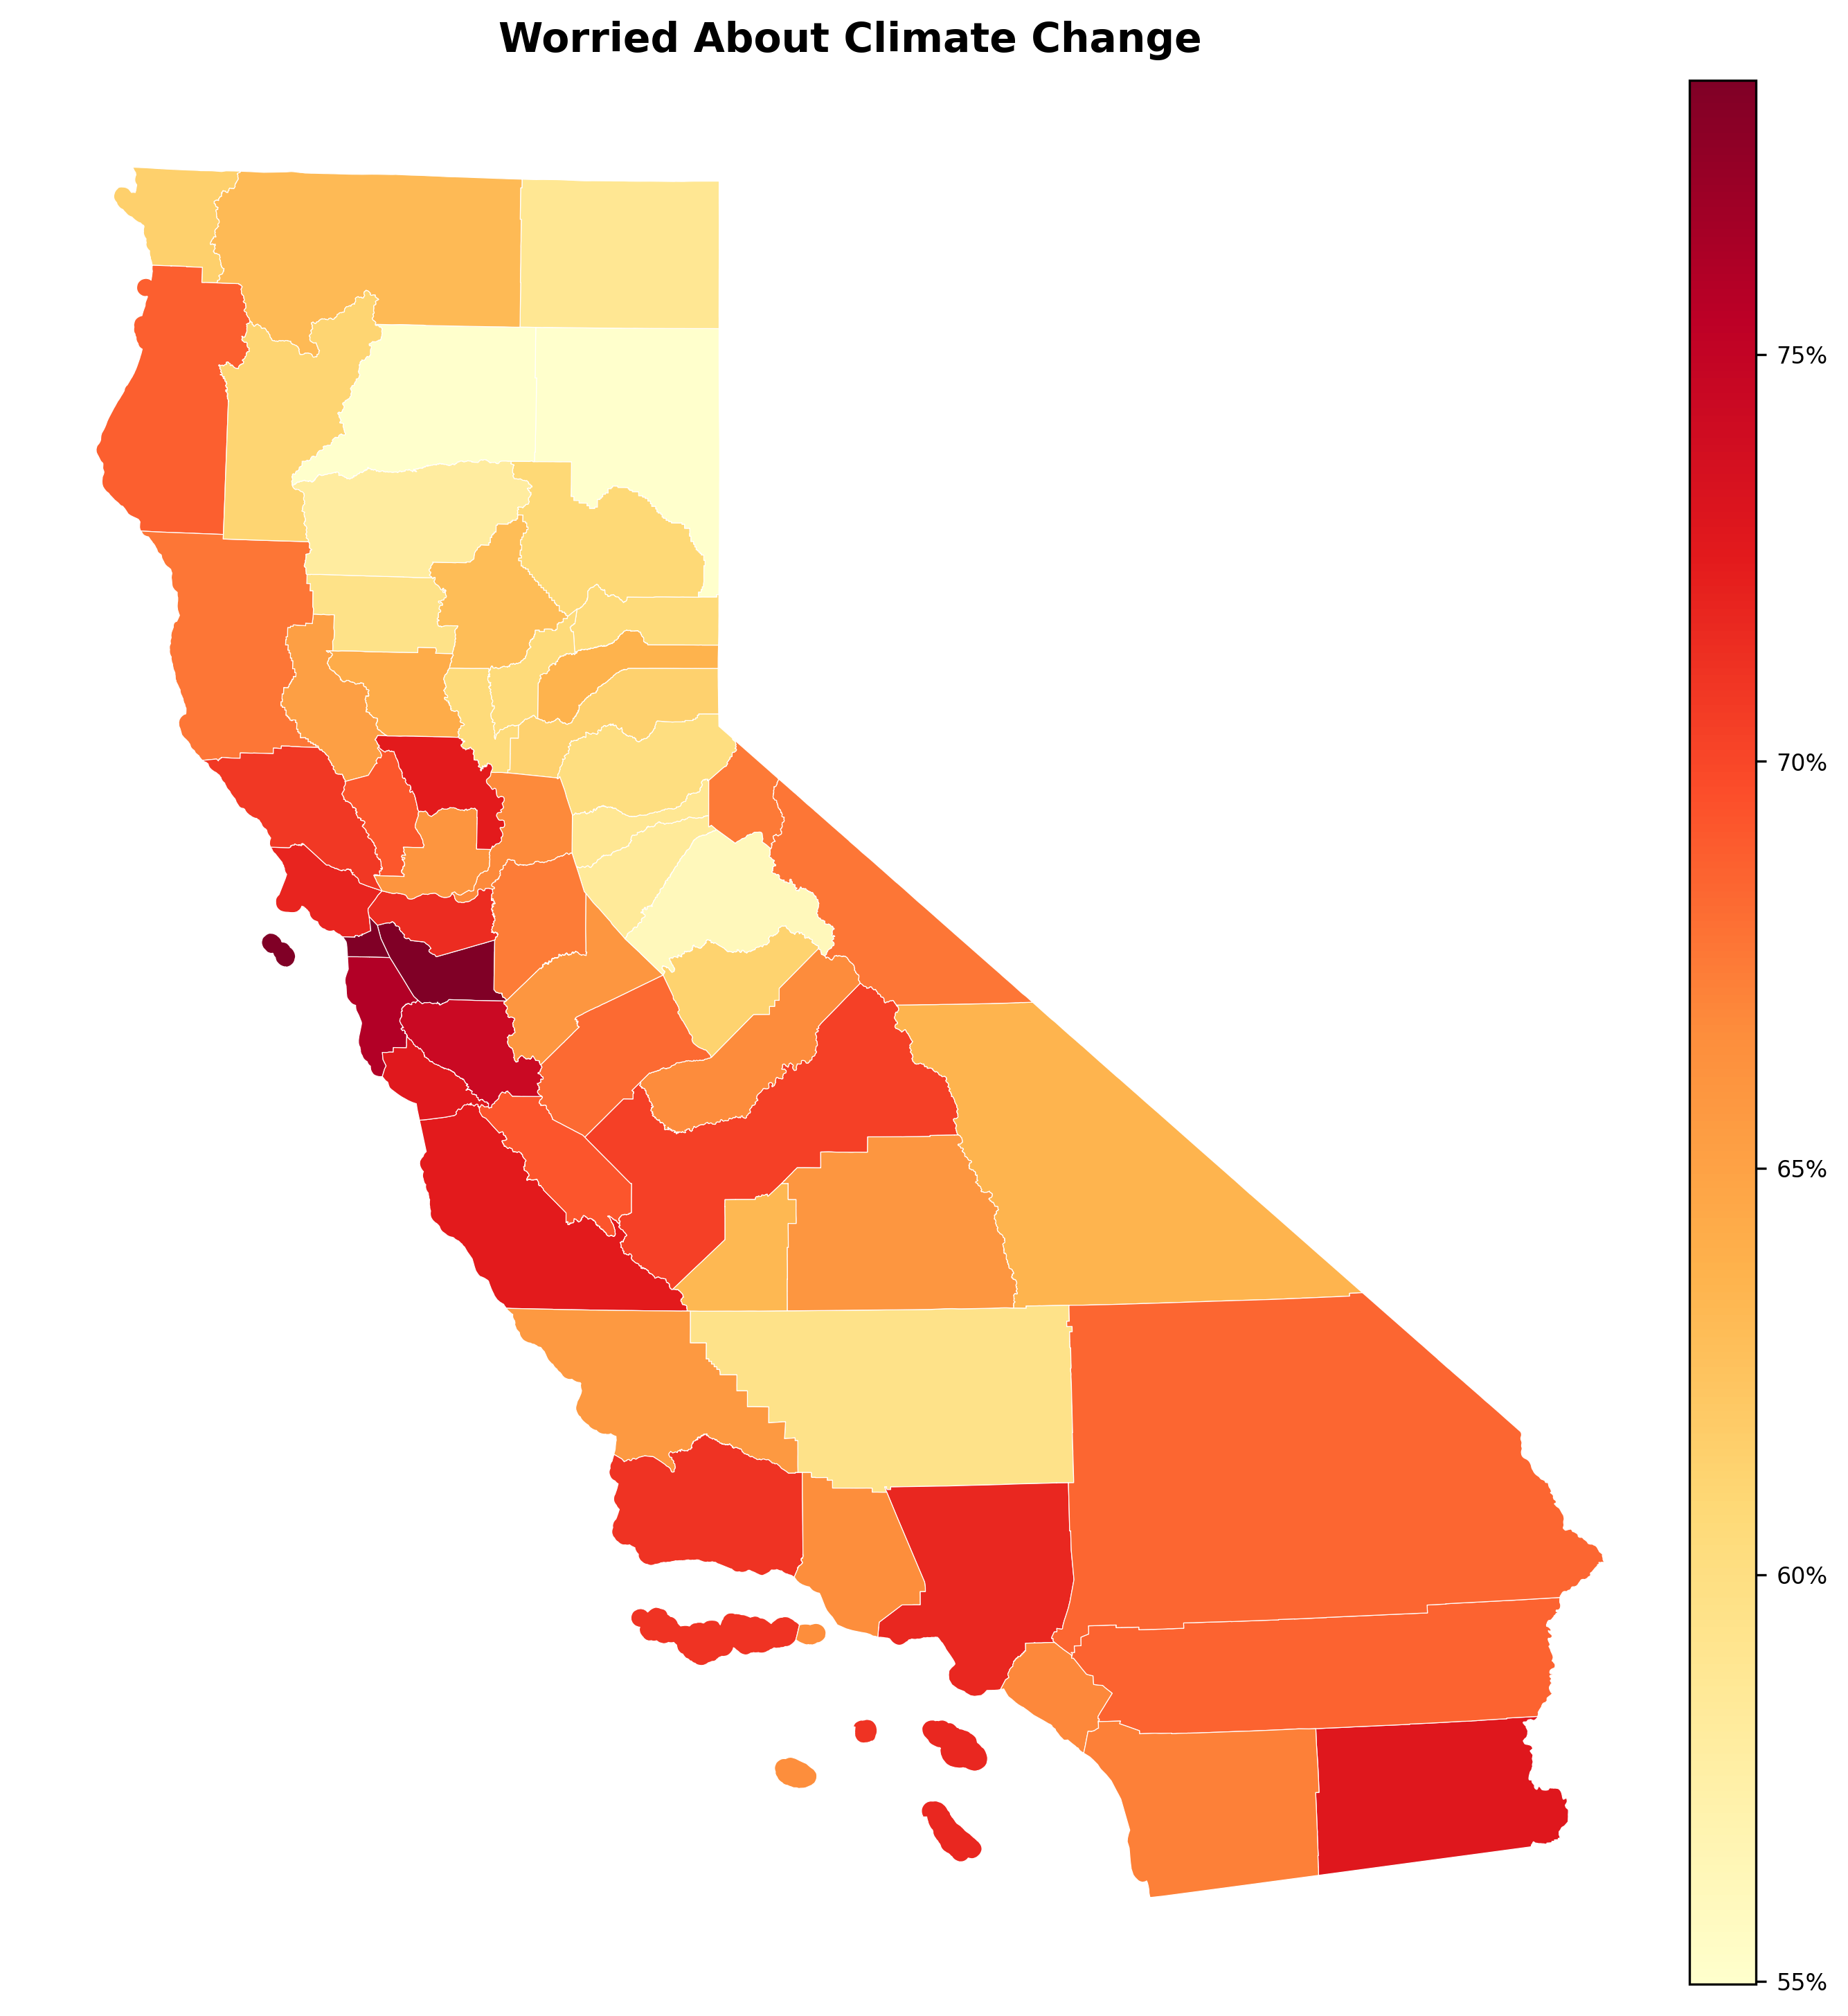
\includegraphics[width=0.80\textwidth]{../output/figures/map_ycom_worried.png}
    }{%
      \missingfig{map\_ycom\_worried.png}
    }
  \end{center}
  \src{Yale Climate Opinion Maps (YCOM), 2023. \% who report being worried about climate change.}
\end{frame}

\begin{frame}{A6: \% Say Climate Change Is Human-Caused (YCOM, County Level)}
  \begin{center}
    \IfFileExists{../output/figures/map_ycom_human.png}{%
      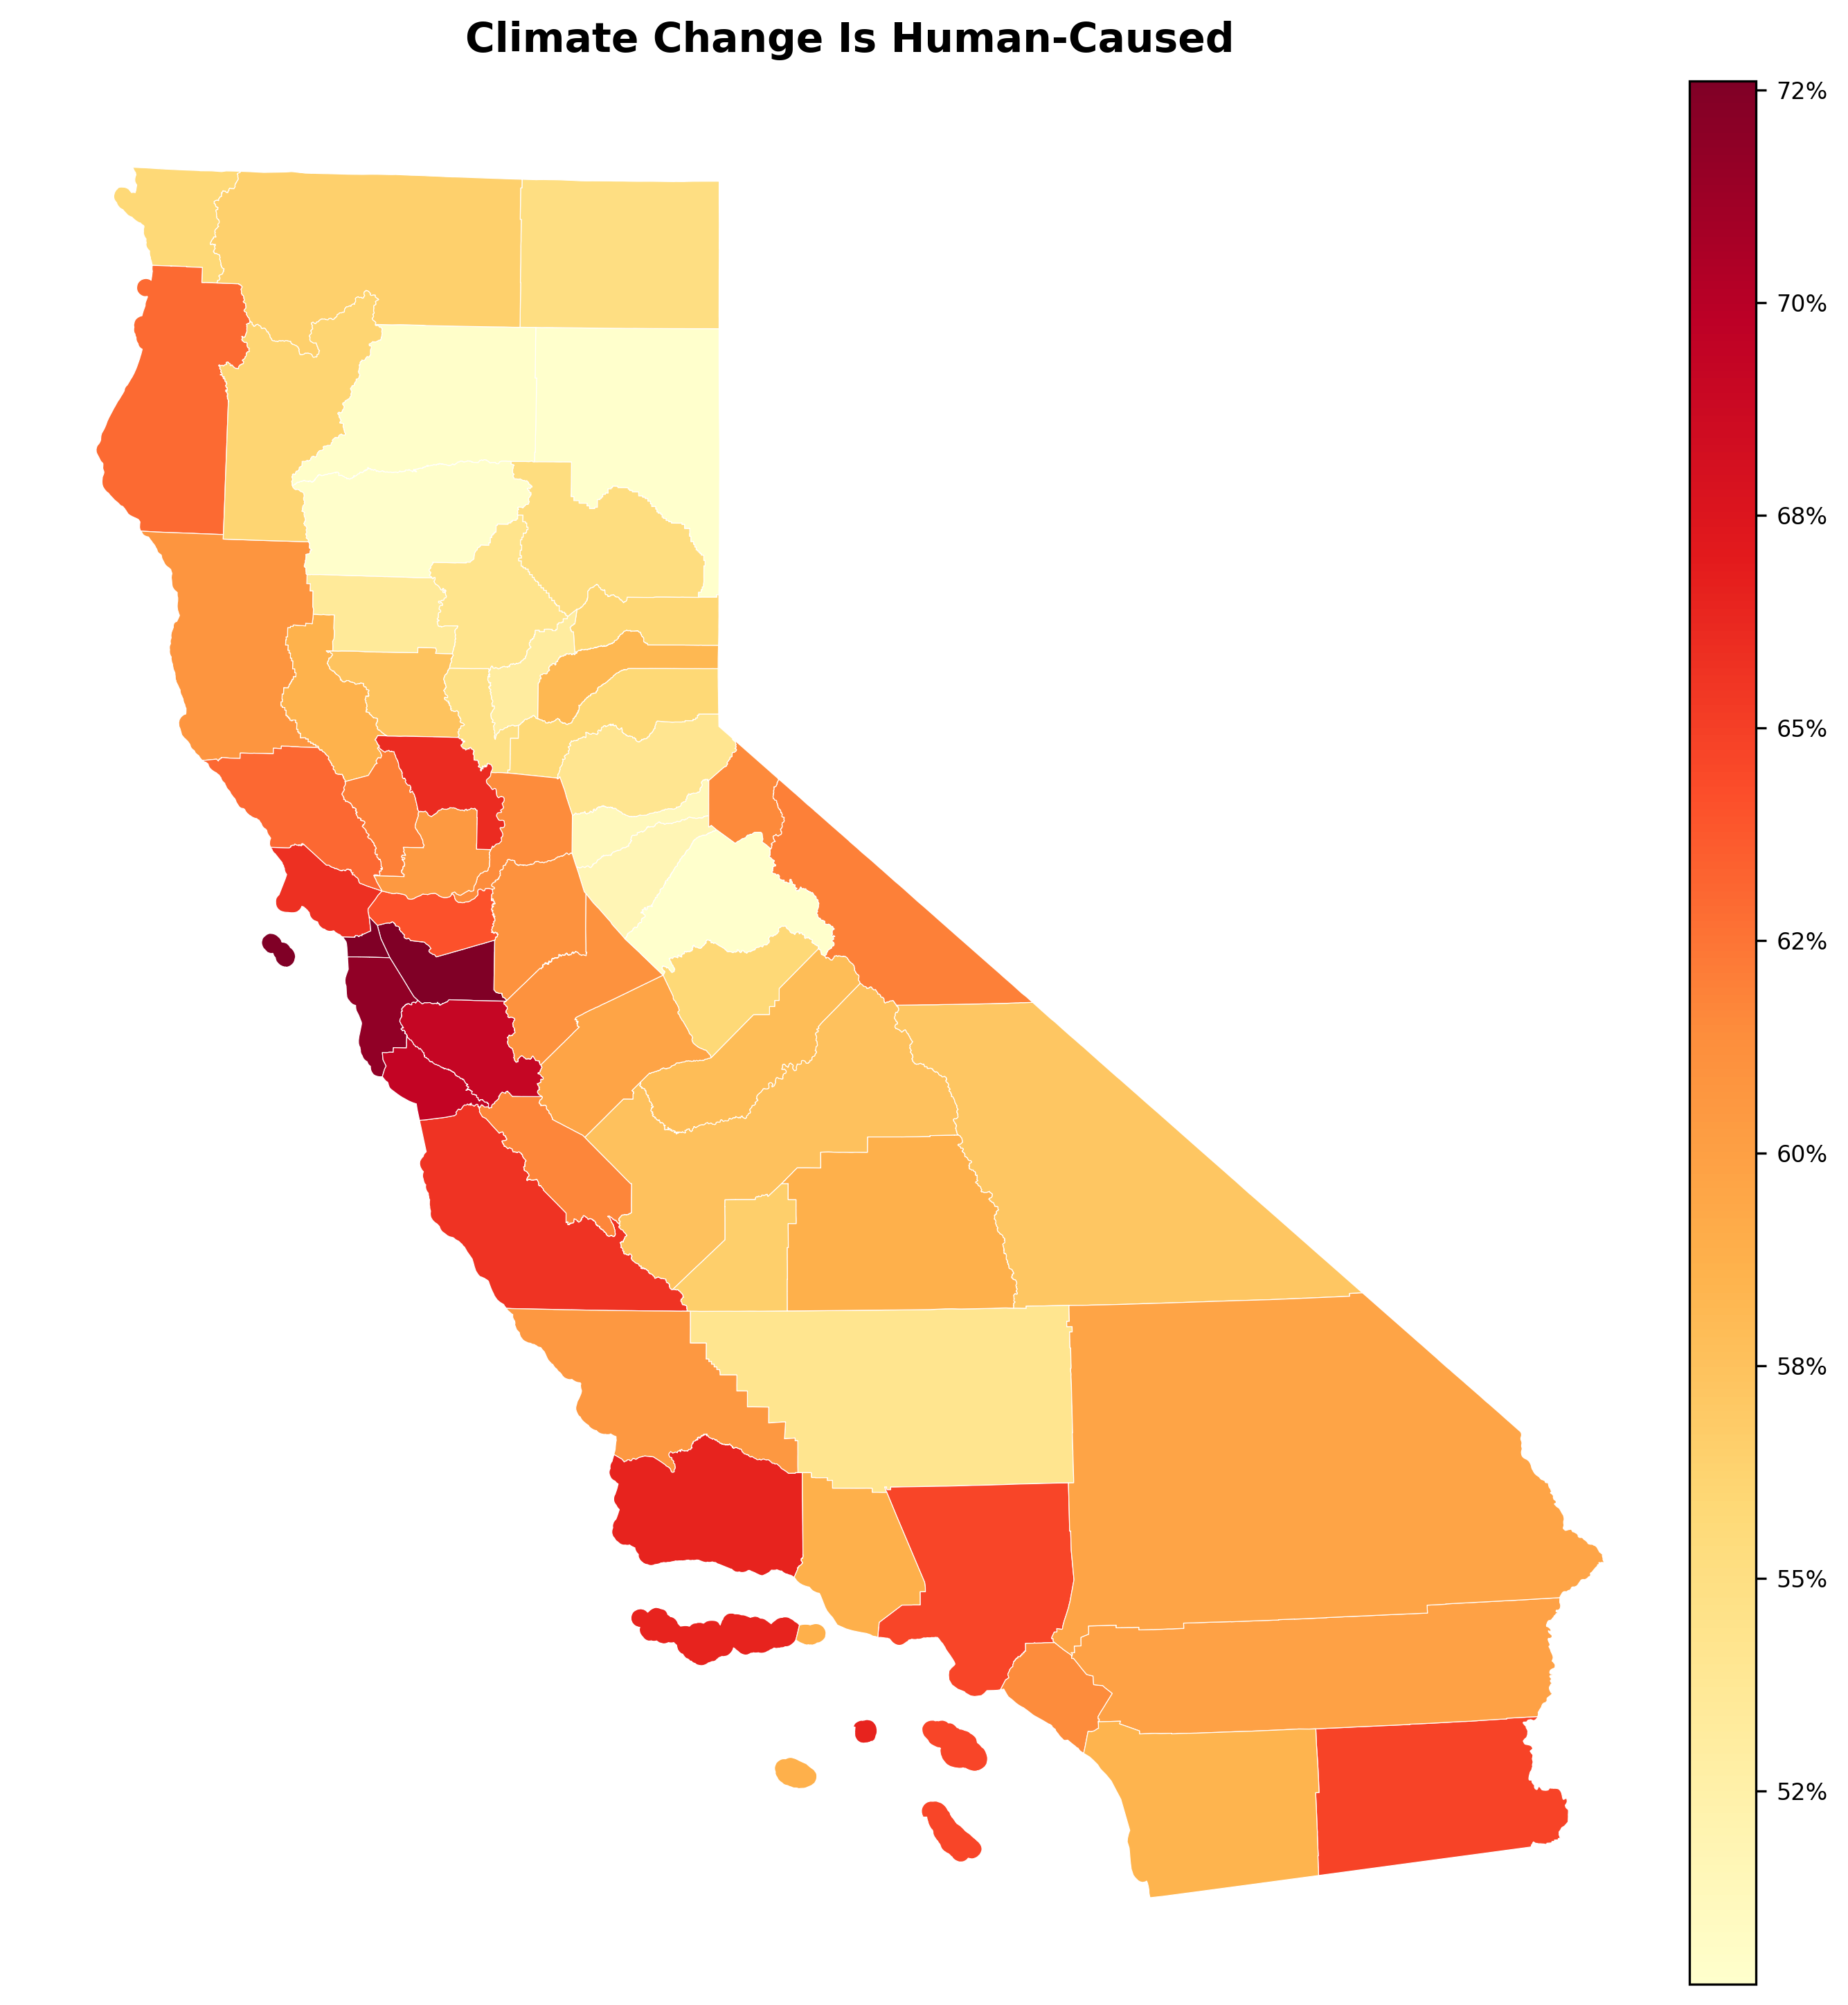
\includegraphics[width=0.80\textwidth]{../output/figures/map_ycom_human.png}
    }{%
      \missingfig{map\_ycom\_human.png}
    }
  \end{center}
  \src{Yale Climate Opinion Maps (YCOM), 2023. \% who attribute climate change primarily to human activity.}
\end{frame}

\begin{frame}{A7: \% Support Climate Regulation (YCOM, County Level)}
  \begin{center}
    \IfFileExists{../output/figures/map_ycom_regulate.png}{%
      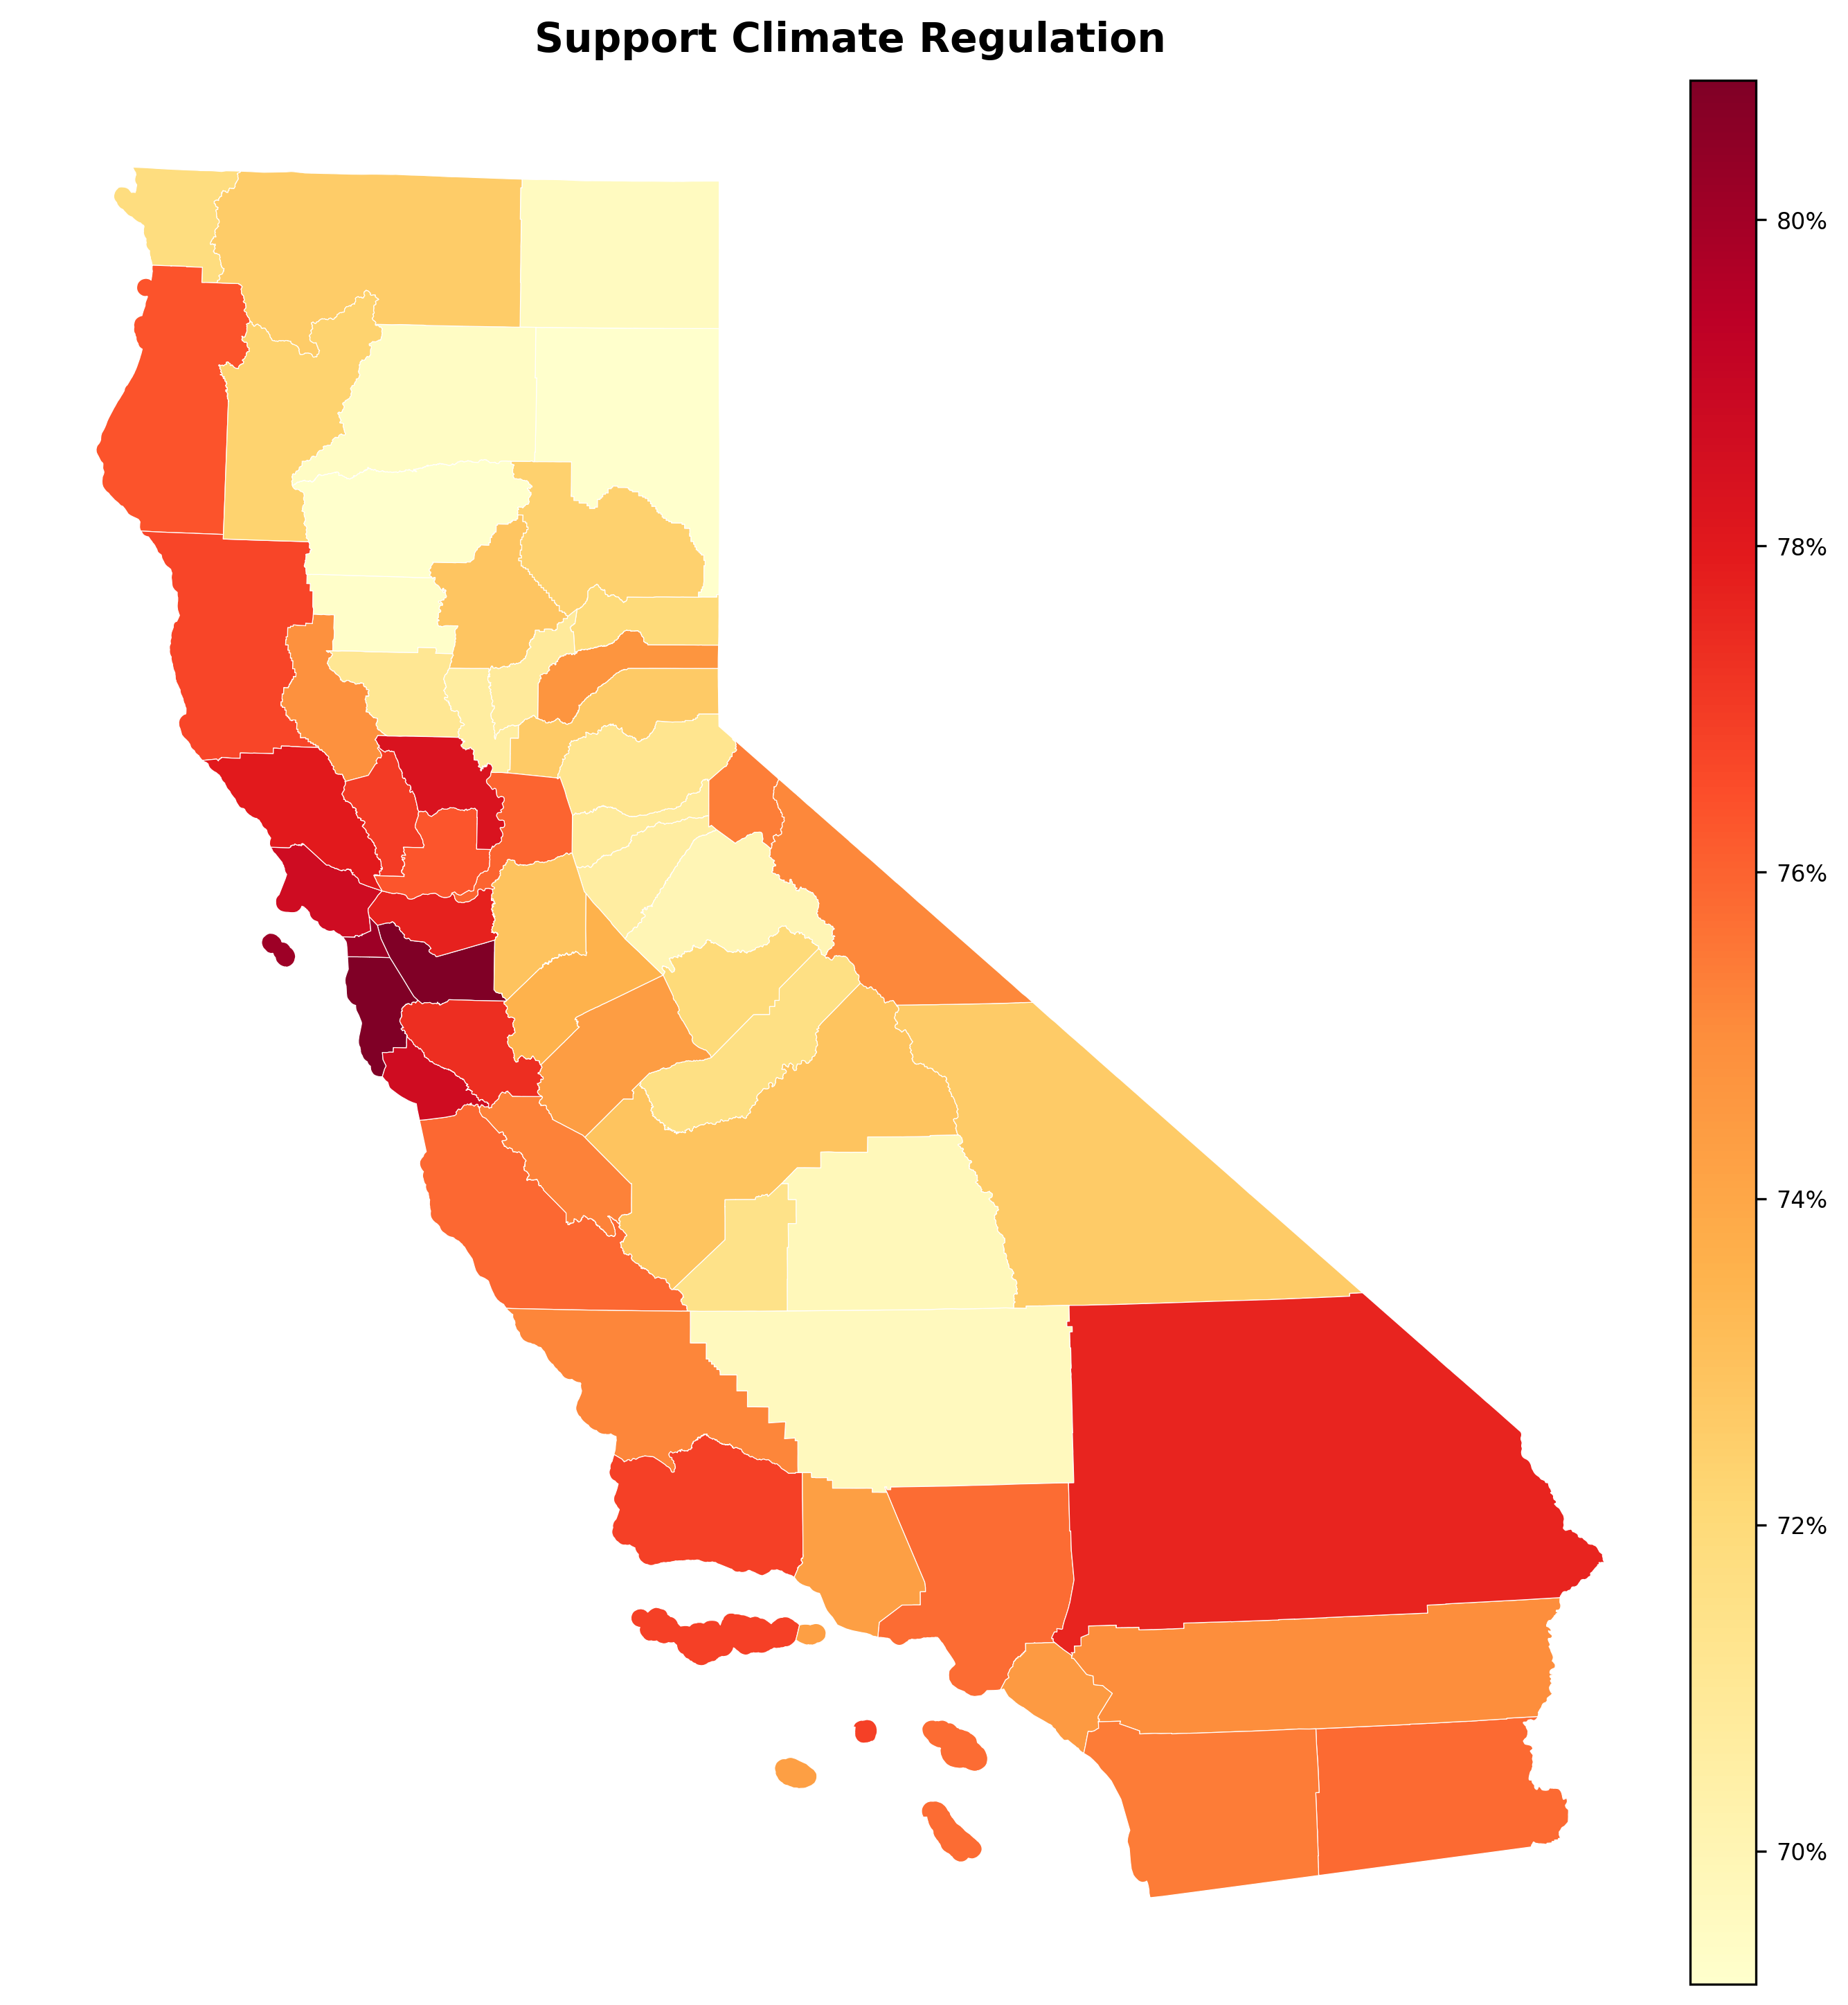
\includegraphics[width=0.80\textwidth]{../output/figures/map_ycom_regulate.png}
    }{%
      \missingfig{map\_ycom\_regulate.png}
    }
  \end{center}
  \src{Yale Climate Opinion Maps (YCOM), 2023. \% who support regulating CO\textsubscript{2} as a pollutant.}
\end{frame}

\begin{frame}{A8: \% Support Renewable Portfolio Standard (YCOM, County Level)}
  \begin{center}
    \IfFileExists{../output/figures/map_ycom_supportRPS.png}{%
      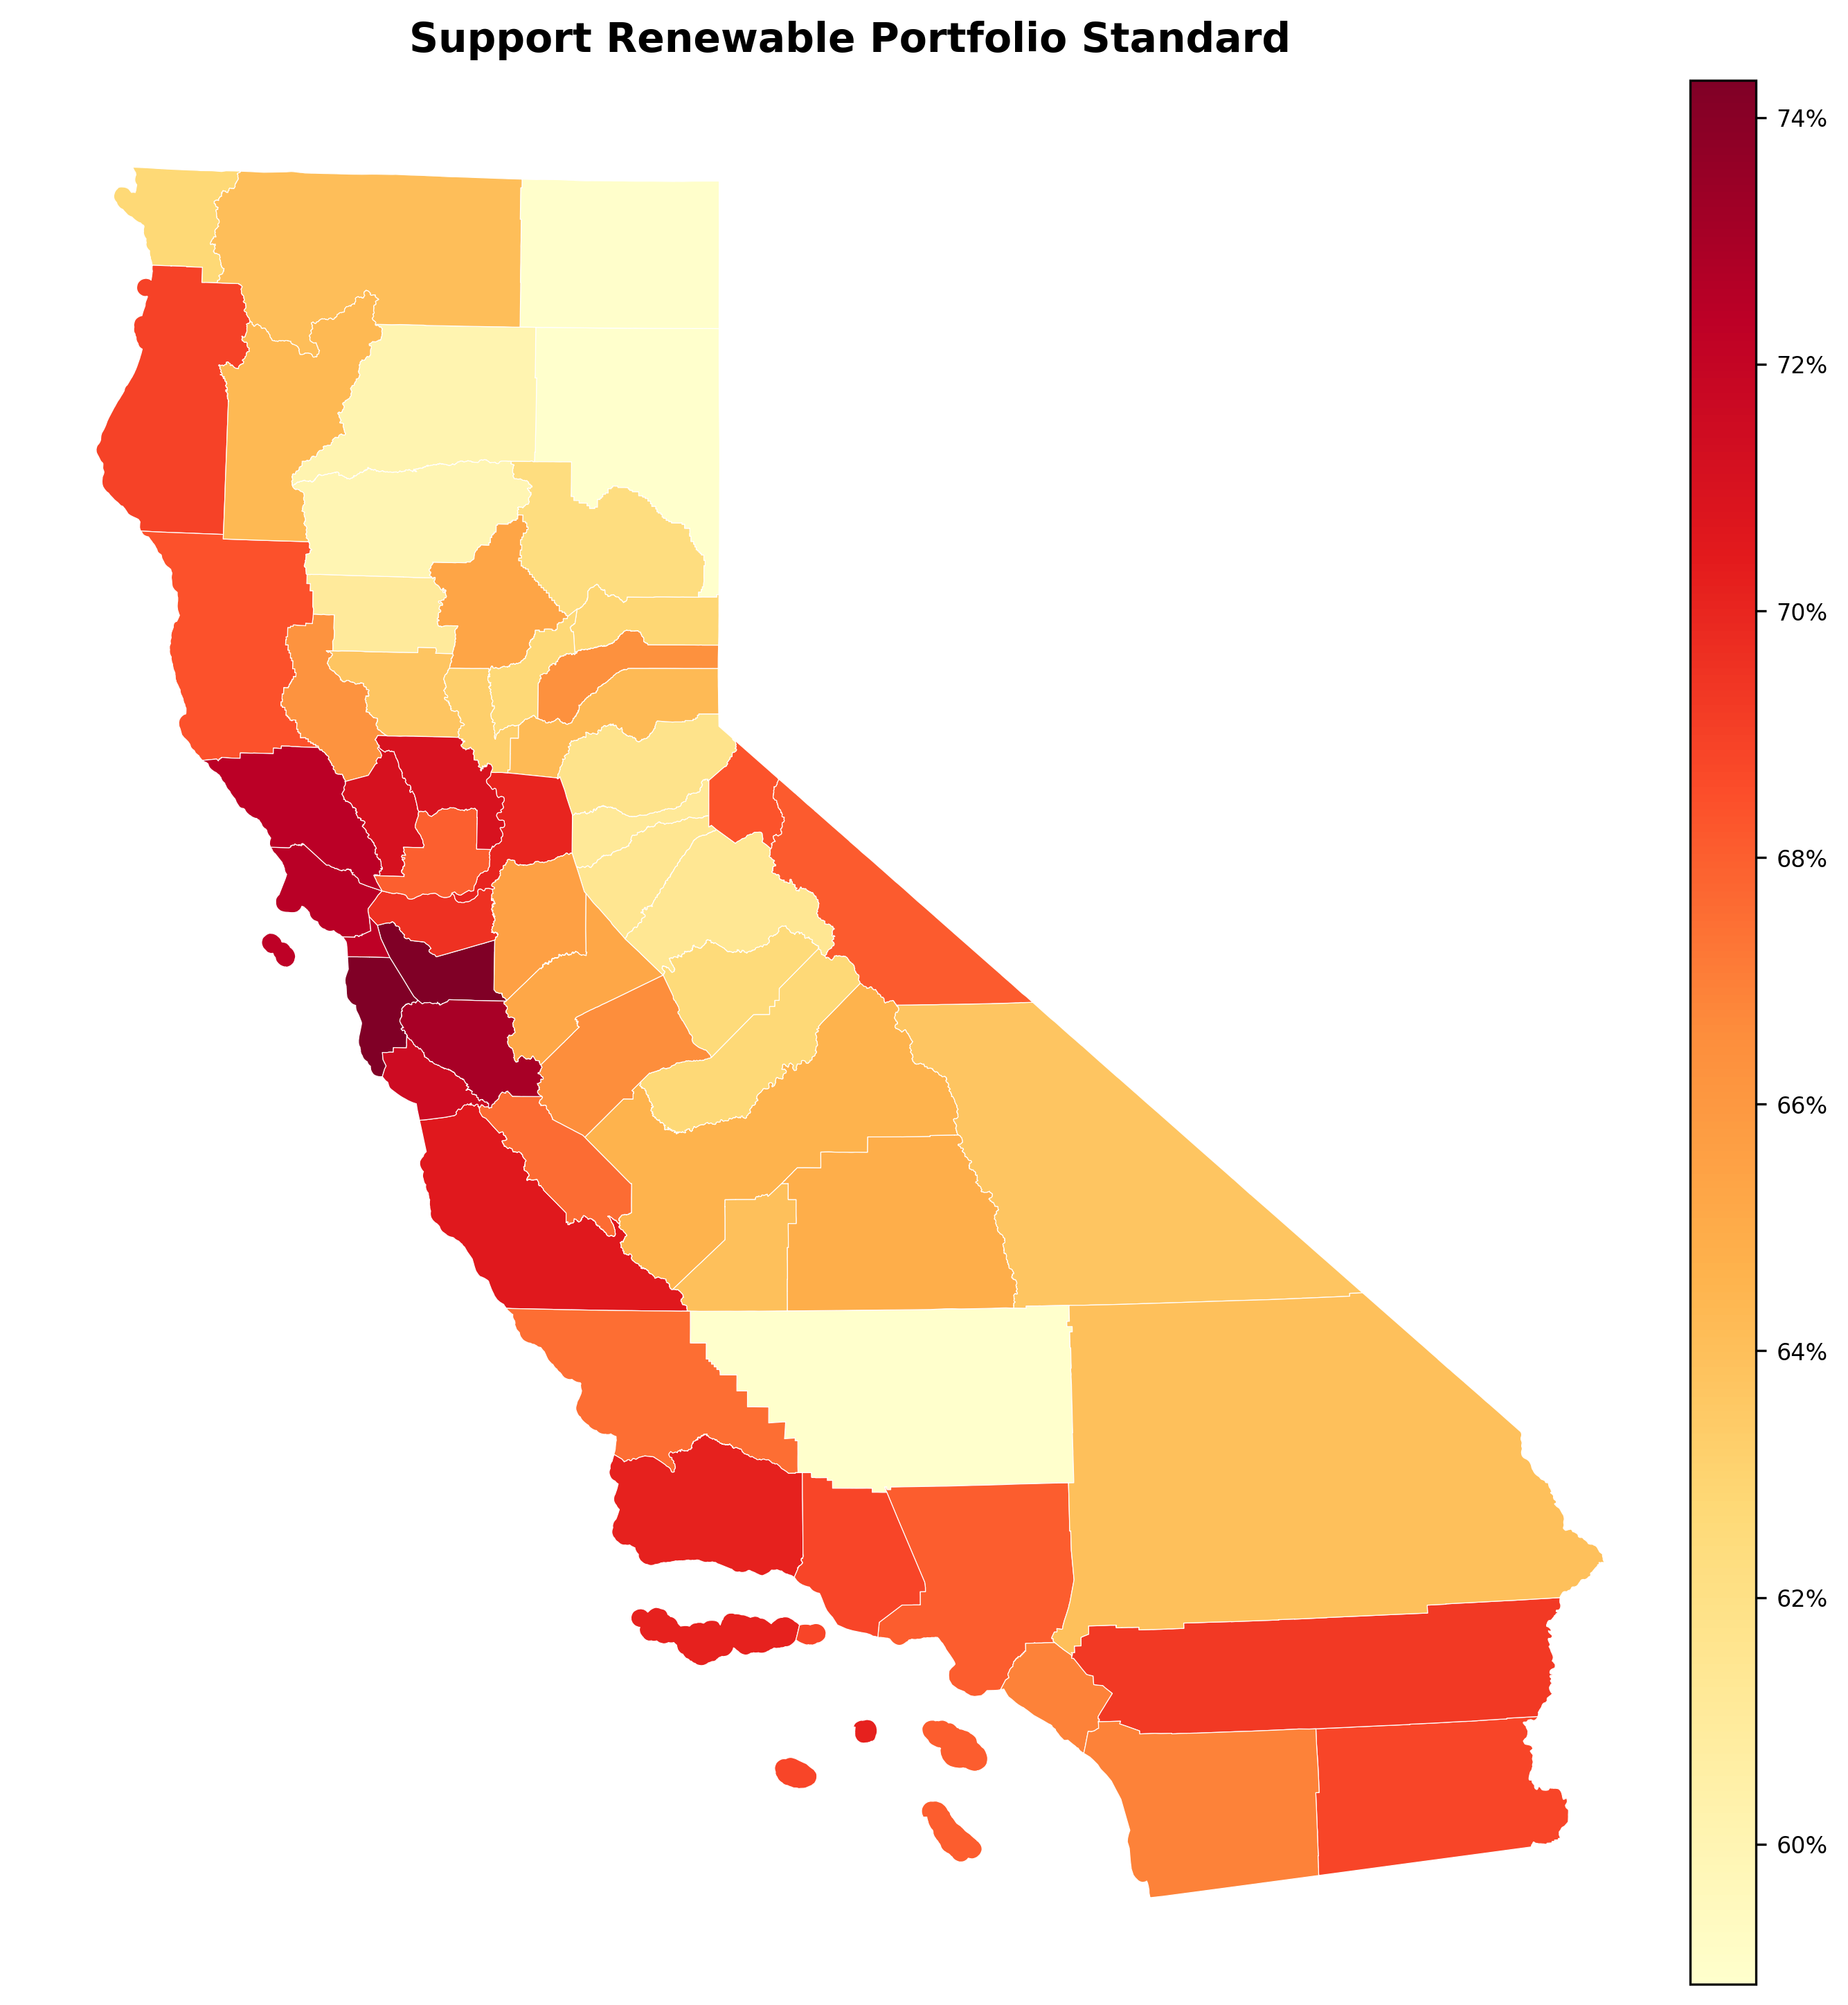
\includegraphics[width=0.80\textwidth]{../output/figures/map_ycom_supportRPS.png}
    }{%
      \missingfig{map\_ycom\_supportRPS.png}
    }
  \end{center}
  \src{Yale Climate Opinion Maps (YCOM), 2023. \% who support requiring utilities to produce electricity from renewable sources.}
\end{frame}

\begin{frame}{A9: Democrat $-$ Republican Registration Share (County Level)}
  \begin{center}
    \IfFileExists{../output/figures/map_dem_minus_rep.png}{%
      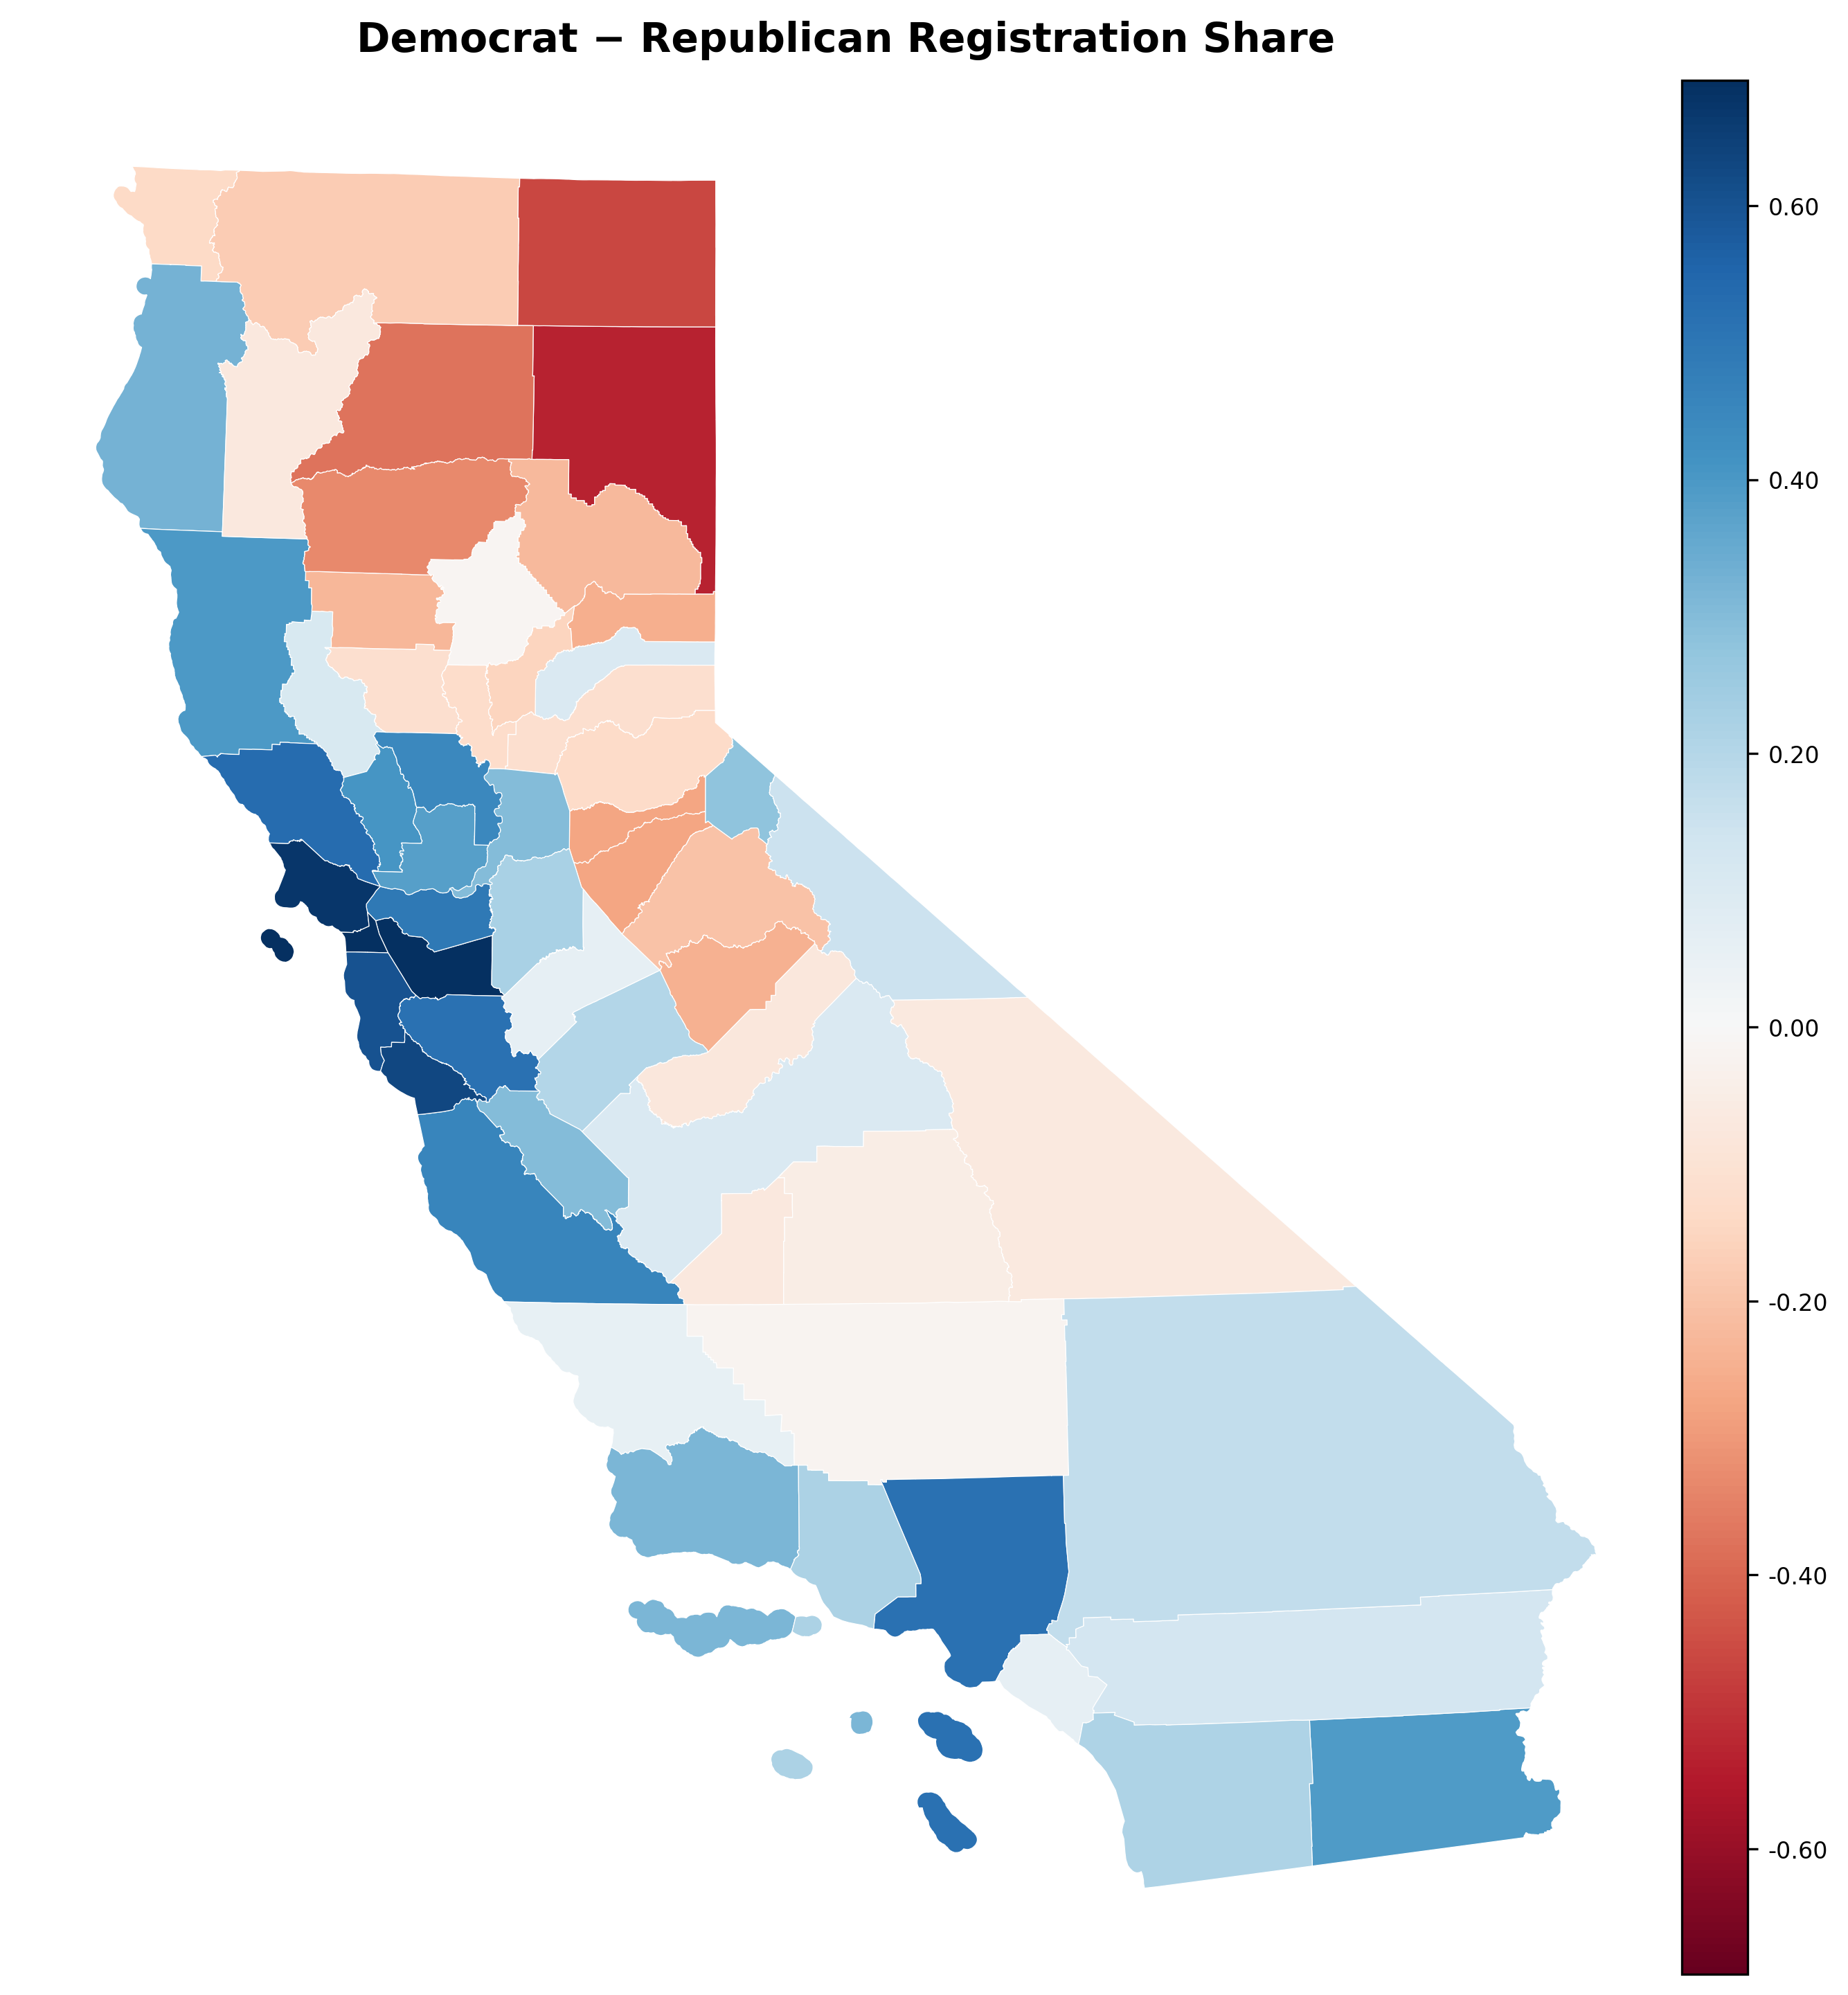
\includegraphics[width=0.80\textwidth]{../output/figures/map_dem_minus_rep.png}
    }{%
      \missingfig{map\_dem\_minus\_rep.png}
    }
  \end{center}
  \src{CA Secretary of State voter registration file (g22 vintage). (DEM $-$ REP) / total registered voters per county.}
\end{frame}

\begin{frame}{A10: Prop 30 YES Share (2022, EV Charging / Wildfire Funding)}
  \begin{center}
    \IfFileExists{../output/figures/map_prop30_yes_share.png}{%
      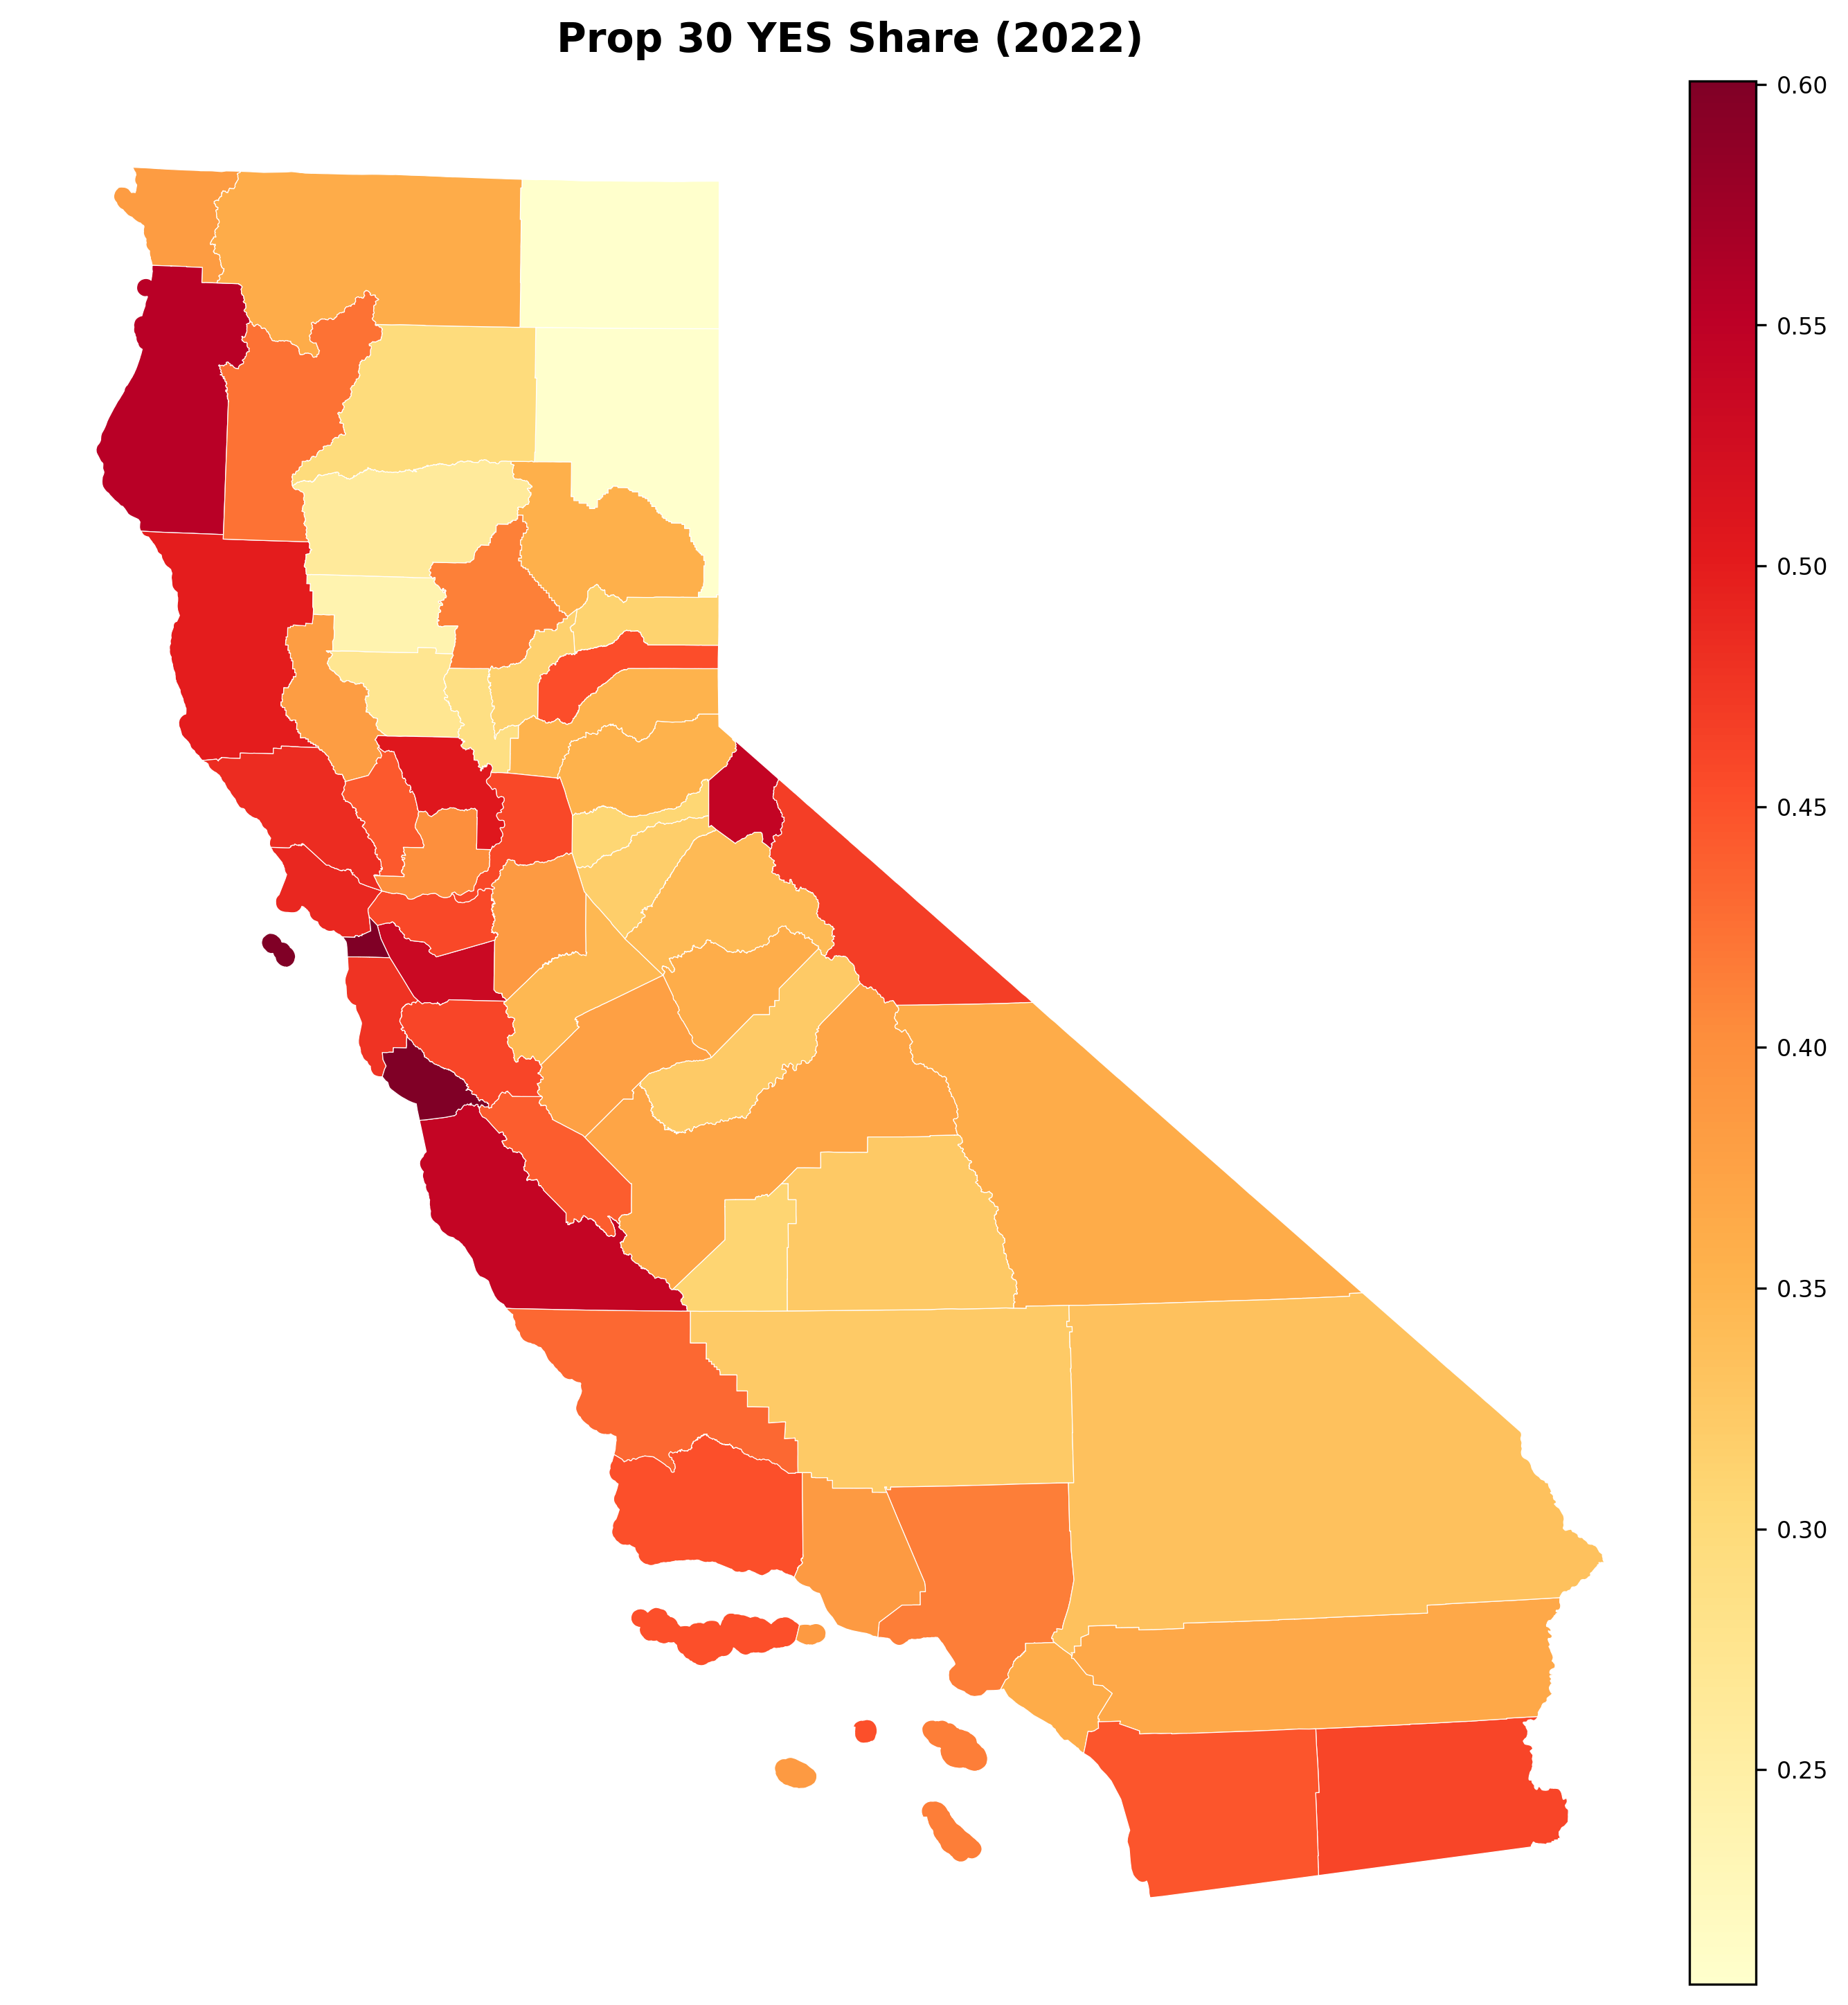
\includegraphics[width=0.80\textwidth]{../output/figures/map_prop30_yes_share.png}
    }{%
      \missingfig{map\_prop30\_yes\_share.png}
    }
  \end{center}
  \src{CA Secretary of State Statement of Vote, November 2022. YES / (YES + NO) per county. Prop 30 proposed a wealth surtax to fund EV infrastructure and wildfire prevention.}
\end{frame}

\begin{frame}{A11: Prop 68 YES Share (2018, Environmental Bonds)}
  \begin{center}
    \IfFileExists{../output/figures/map_prop68_yes_share.png}{%
      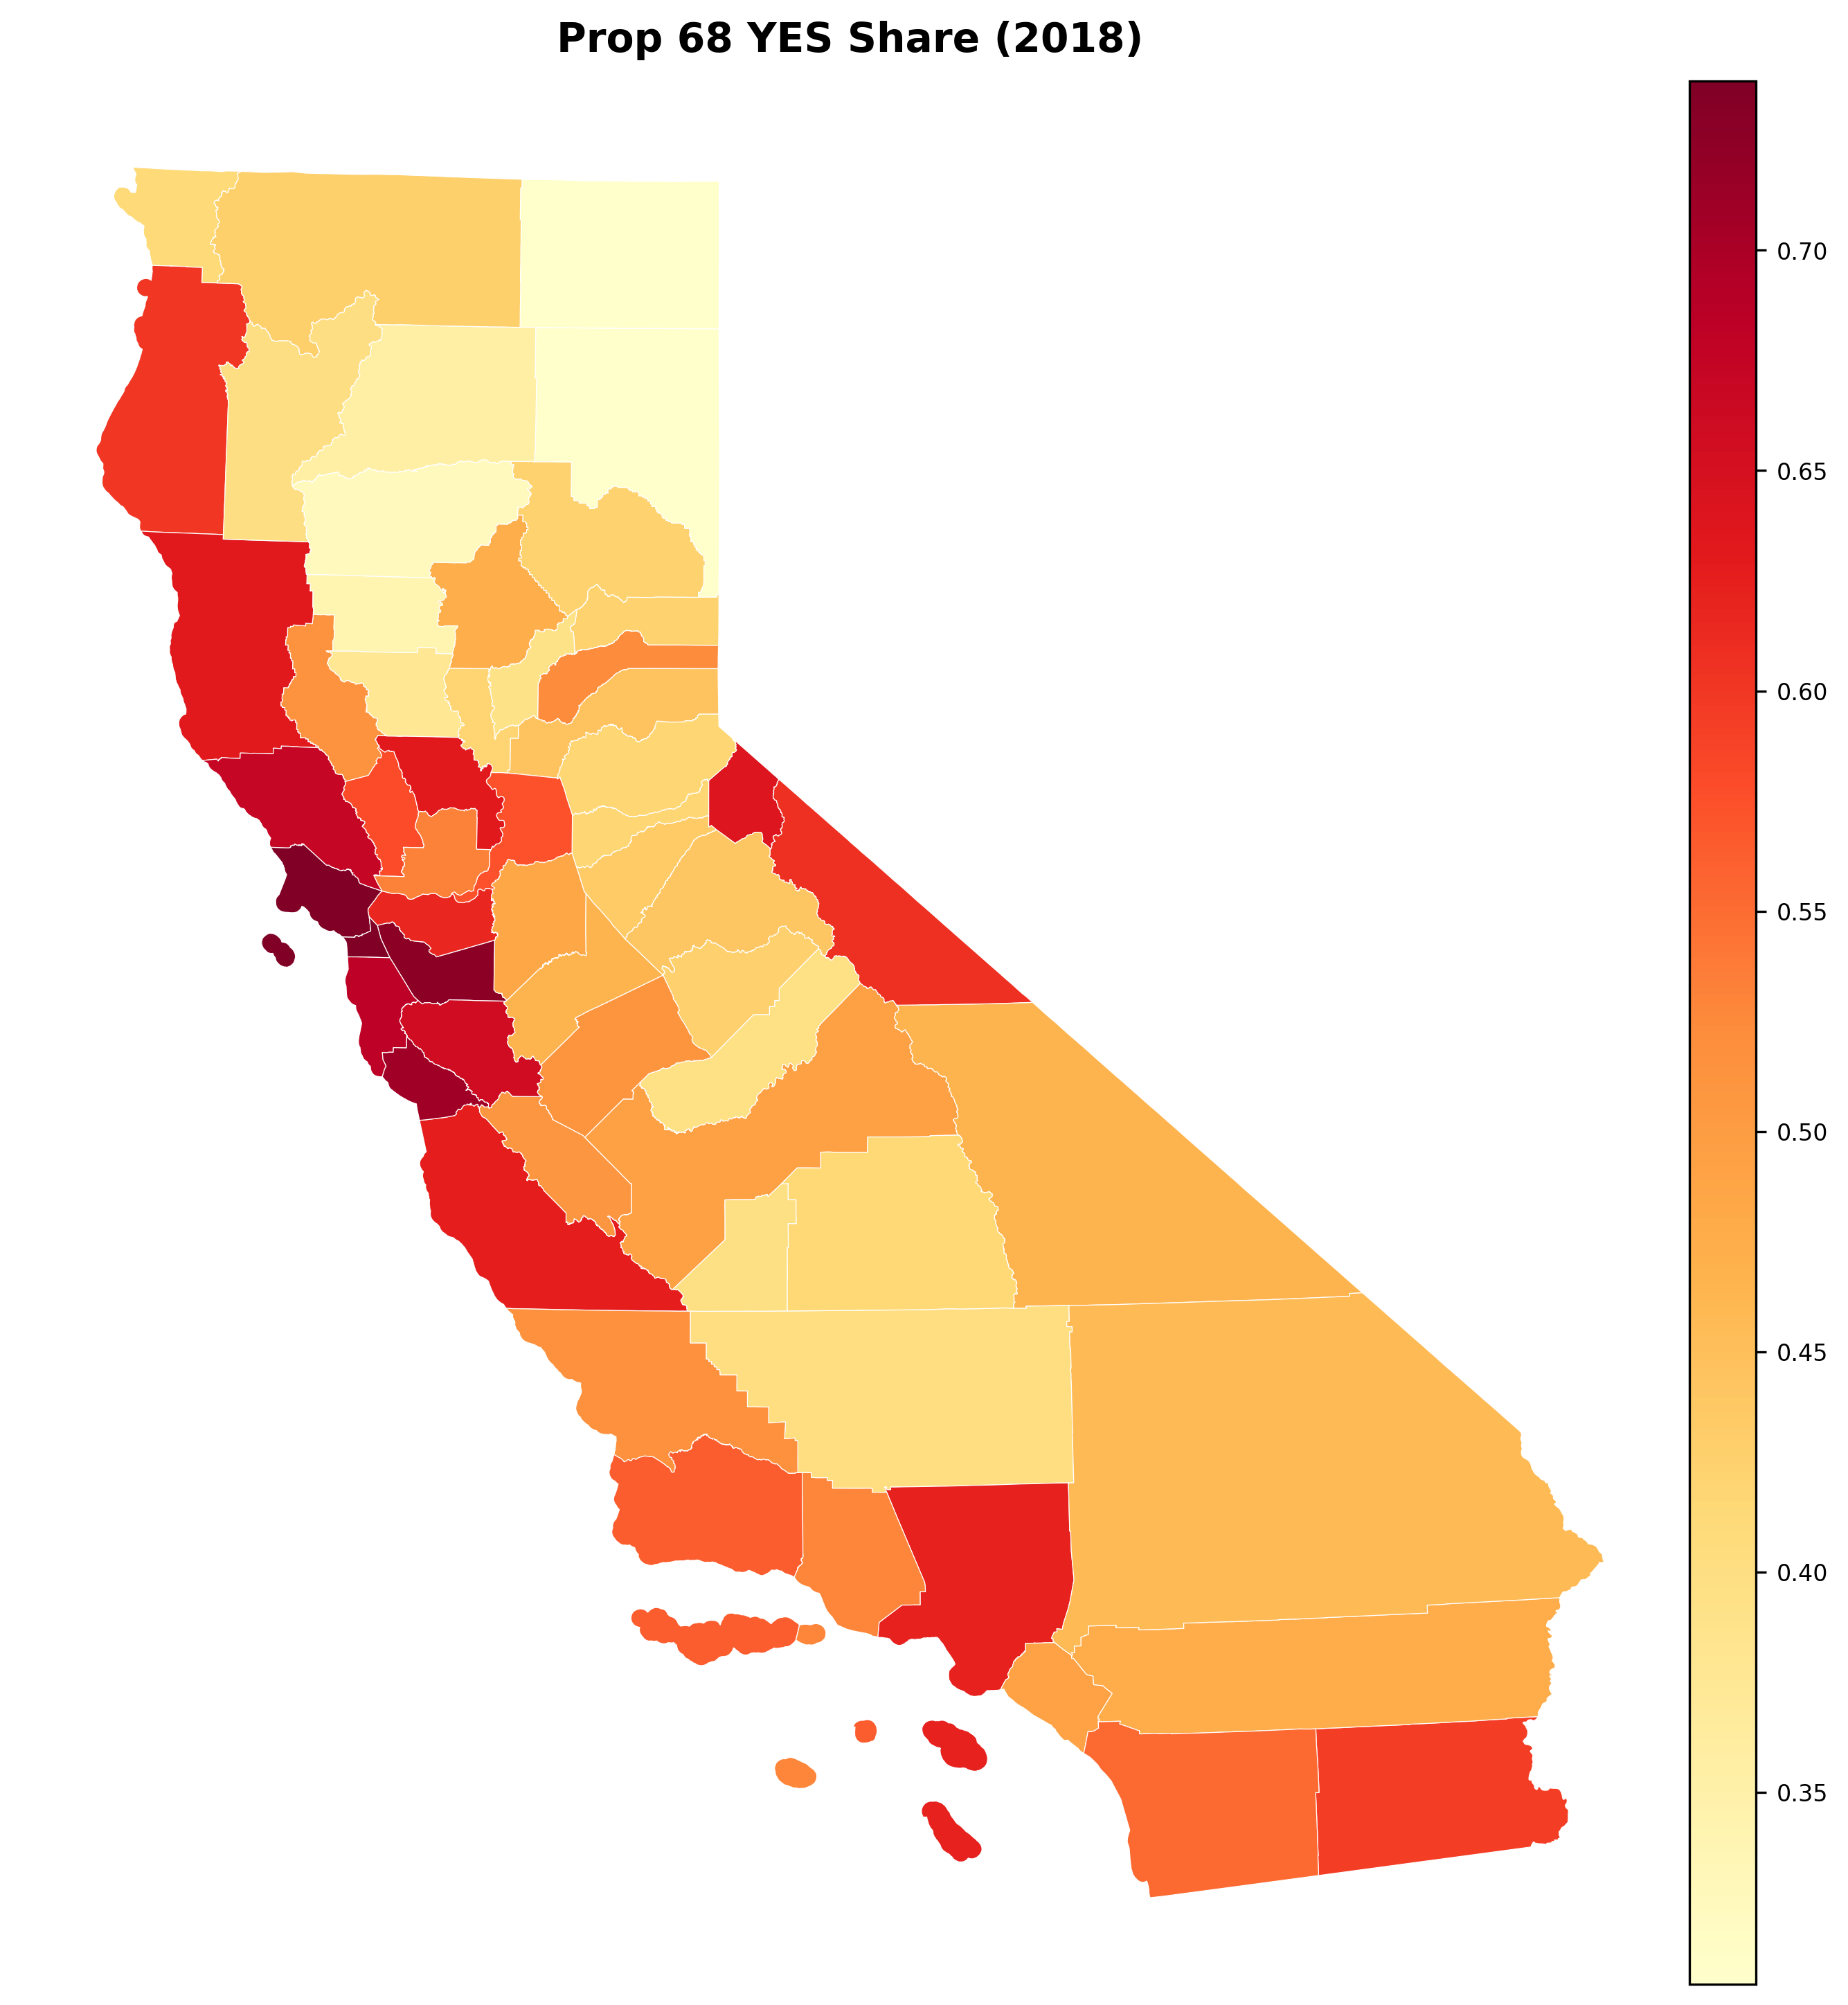
\includegraphics[width=0.80\textwidth]{../output/figures/map_prop68_yes_share.png}
    }{%
      \missingfig{map\_prop68\_yes\_share.png}
    }
  \end{center}
  \src{CA Secretary of State Statement of Vote, June 2018 Primary. YES / (YES + NO) per county. Prop 68 authorized \$4B in bonds for parks, environmental protection, and water projects.}
\end{frame}

\begin{frame}{A12: Placebo Check — Light Truck Event Study}
  \begin{center}
    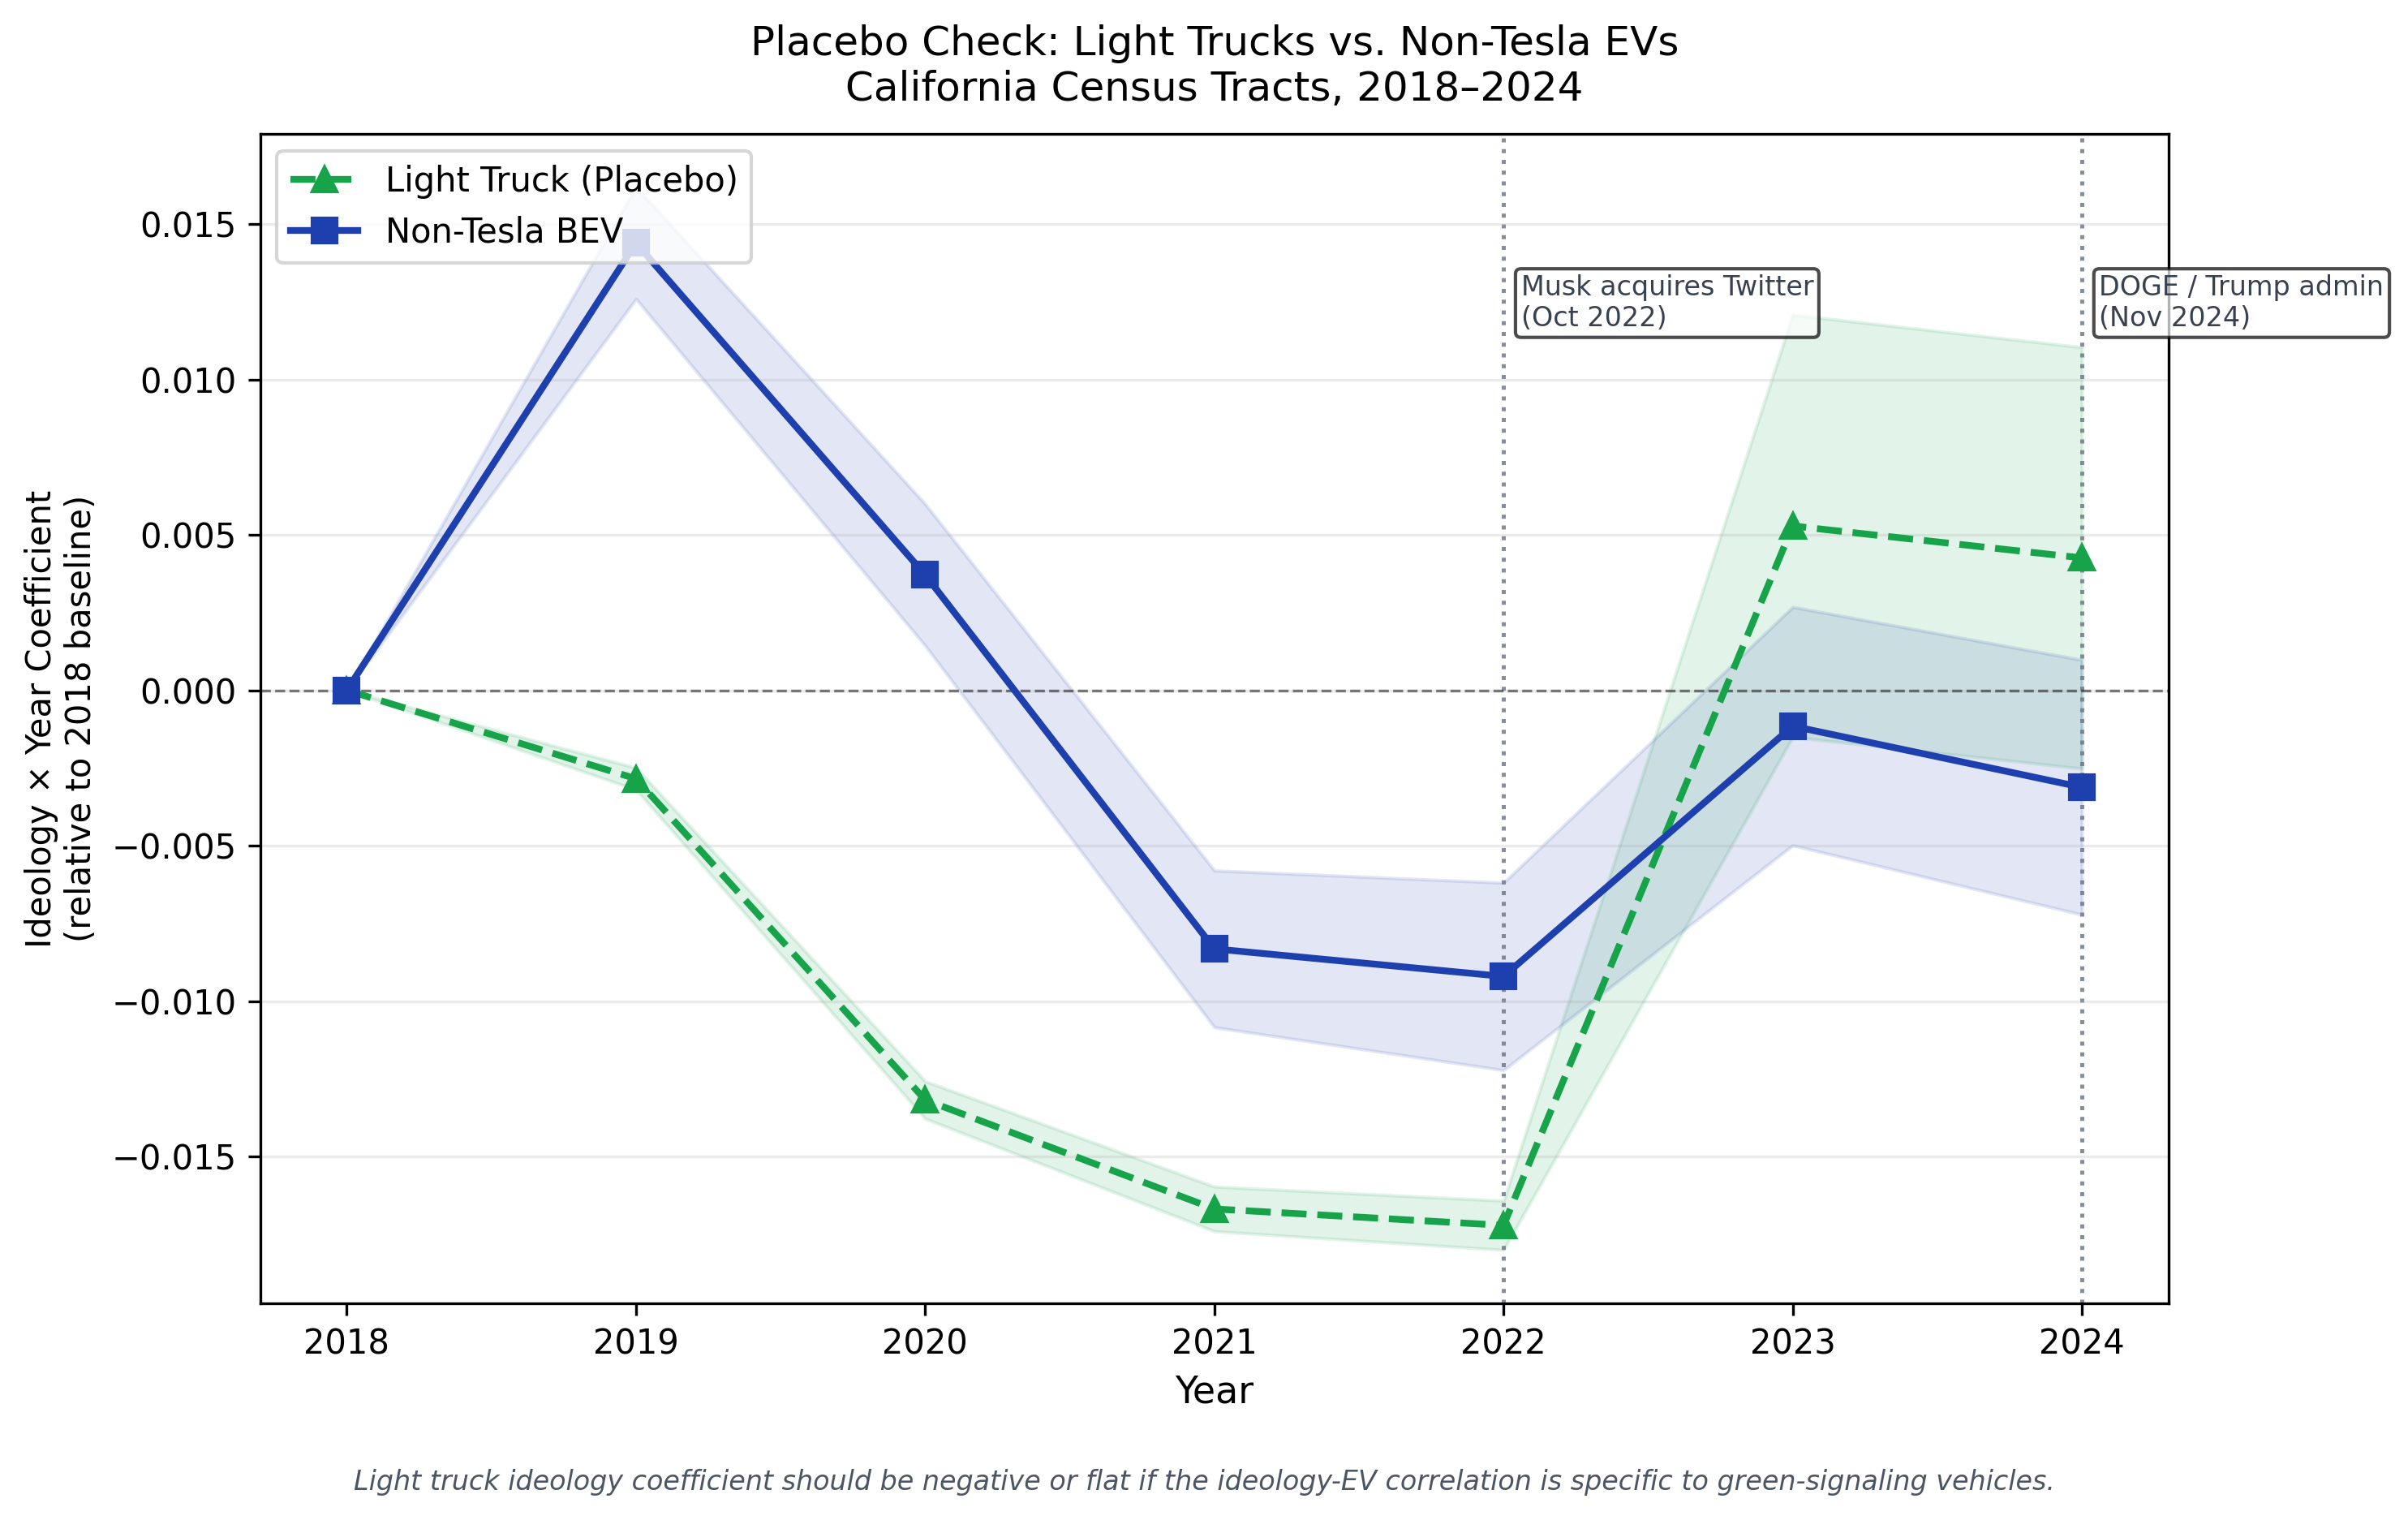
\includegraphics[width=0.82\textwidth]{../output/figures/event_study_truck_placebo.png}
  \end{center}
  \vspace{-0.4em}
  \src{Ideology $\times$ year coefficients for light trucks (green, dashed) vs.\ non-Tesla BEVs (blue).
  A rising truck line post-2022 would indicate climate-conscious communities shifting away from EVs broadly. The monotone truck decline (2019--2022) is distinct from both EV series and consistent with the truck boom being a low-ideology phenomenon.}
\end{frame}

\end{document}
